% CS5494 Assignment report
% Typography follows the CityUHK thesis template conventions (XeLaTeX, Times New Roman,
% A4, plain page style with centred page numbers, black hyperlinks).
\documentclass[11pt,a4paper]{article}

\usepackage{fontspec}
\setmainfont{Times New Roman}
% SimSun is used only for the Chinese form of the author name on the title page; Times New Roman
% has no CJK glyphs. Remove this line and the {\zhfont ...} group below for a Latin-only name.
\newfontfamily\zhfont{SimSun}
\usepackage[margin=2.5cm]{geometry}
\usepackage{amsmath,amssymb}
\usepackage{booktabs}
\usepackage{graphicx}
\usepackage{float}
\usepackage{caption}
\usepackage{subcaption}
\usepackage{array}
\usepackage{enumitem}
\usepackage[backend=biber,style=authoryear,maxcitenames=2]{biblatex}
\usepackage[colorlinks=true,linkcolor=black,citecolor=black,urlcolor=black]{hyperref}
\usepackage{fancyhdr}
\usepackage{siunitx}
\usepackage{listings}
\lstset{
  language=Python,
  basicstyle=\ttfamily\scriptsize,
  breaklines=true,
  breakatwhitespace=false,
  showstringspaces=false,
  tabsize=4,
  columns=flexible,
  keepspaces=true
}

\pagestyle{fancy}
\fancyhf{}
\fancyfoot[C]{\thepage}
\renewcommand{\headrulewidth}{0pt}

\clubpenalty10000
\widowpenalty10000
\captionsetup{font=small,labelfont=bf}
\setlist{itemsep=2pt,topsep=3pt}
\sisetup{detect-weight=true,group-separator={,}}

\addbibresource{refs.bib}

\newcommand{\outputs}{\texttt{outputs\_final}}

\title{\bfseries Autoregressive and Adversarial Generative Models for MNIST}
\author{Name: {\zhfont 刘纳多} (LIU Naduo) \quad Student ID: 60777841\\
\small Code and data (GitHub, public): \url{https://github.com/Minnesinger02/CS5494AS1}}
\date{CS5494 Topics in Generative AI --- Assignment, November 2026\\[2pt]
\small Training data: the entire 60{,}000-image MNIST training set
(binarised for FVSBN and MADE; grayscale for the GAN)}

\begin{document}
\maketitle

\begin{abstract}
\noindent
This report implements the three generators required by the assignment: a fully visible
sigmoid belief network, a neural autoregressive model, and a generative adversarial network
on MNIST. All autoregressive models are trained on $28\times28$ binarised digits and evaluated
by exact held-out likelihood, reported both as nats per image and as bits per pixel so that
results at different resolutions remain comparable. The generative adversarial network is
trained on the original grayscale digits and evaluated with an independent classifier.
Beyond the baseline implementations we report a validation-based hyperparameter study of the
autoregressive model, a three-member mixture of autoregressive models, a convolutional
adversarial architecture with a two-timescale update rule, and an exponential moving average
of the generator weights. The final autoregressive model reaches $0.1223$ bits per pixel as a
three-member mixture ($0.1260$ for a single model), and the convolutional generator reaches a
feature-Fr\'echet distance of 7.12 against 34.61 for the initial fully connected baseline.
\end{abstract}

\newpage
\tableofcontents
\newpage
%----------------------------------------------------------------------------------------
\section{Introduction}
%----------------------------------------------------------------------------------------

The assignment asks for three separate image generators on MNIST~\parencite{mnist1998}.
Section~1.1 requires a \emph{fully visible} sigmoid belief network, that is, a model with no
latent or hidden variables whose conditionals are logistic; Section~1.2 requires a
\emph{neural} autoregressive model with one or more layers; Section~1.3 requires a generative
adversarial network trained on the original, non-binarised digits, together with a short
discussion of training stability.
The two autoregressive models are trained on binarised digits, the generative adversarial
network on grayscale digits, and each model is evaluated on the metric that its formulation
supports: exact likelihood for the autoregressive models and a classifier-based distribution
distance for the adversarial one.

The report makes four additions to a straightforward implementation.
First, the autoregressive inputs use the full $28\times28$ resolution rather than a reduced
grid, which lowers the cost per pixel by roughly a factor of two even though the total
per-image likelihood rises.
Second, the capacity, depth and regularisation of the autoregressive network were selected on
a held-out slice of the \emph{training} set, so the test set is read only once.
Third, three independently seeded autoregressive models are combined into a mixture, and the
effect of the mixture size is measured rather than assumed.
Fourth, the adversarial model is first trained as a fully connected baseline, then as a
convolutional network with a two-timescale update rule, and finally with an exponential moving
average of the generator weights; each change is reported with the same three external
statistics, which makes the improvement traceable rather than anecdotal.

%----------------------------------------------------------------------------------------
\section{Data and preprocessing}
%----------------------------------------------------------------------------------------

MNIST contains 60{,}000 training and 10{,}000 test images of size $28\times28$ with pixel
intensities $v\in\{0,\dots,255\}$.
For the two autoregressive models the digits are binarised with a fixed threshold,
\begin{equation}
  x_{ij} = \mathbf{1}\left[\frac{v_{ij}}{255} \ge 0.5\right],
  \label{eq:binarise}
\end{equation}
which yields a mean ink coverage of $13.2\%$ over the training set; a pixel is therefore much
more likely to be background than stroke, and a model that only predicts the marginal
distribution already reaches $0.5636$ bits per pixel.
No resizing is applied, so the autoregressive input is a $784$-dimensional binary vector in
raster order. A $14\times14$ variant with the same threshold is included as a resolution
reference in Section~\ref{sec:discussion} and stored under \texttt{results/ablation\_14x14}.
For the generative adversarial network the digits keep their grayscale values and are scaled
to $[-1,1]$, which matches the $\tanh$ output of the generator.

The training subset is drawn once with \texttt{torch.randperm} under seed~42 and stored with
each run, so every experiment that uses the same number of images sees exactly the same
digits. The $10{,}000$-image ablation reuses the first $10{,}000$ entries of that permutation.
Hyperparameter selection used a further split of $5{,}000$ images taken from the \emph{front}
of the training subset; those images were never used for gradient updates while tuning, and
the final models are retrained on all $60{,}000$ images with the selected settings.
The test set is used exclusively for the numbers reported in Section~\ref{sec:experiments}.

%----------------------------------------------------------------------------------------
\section{Methods}
%----------------------------------------------------------------------------------------

\subsection{Fully visible sigmoid belief network}
\label{sec:fvsbn}

The fully visible sigmoid belief network factorises the joint distribution into one logistic
conditional per pixel,
\begin{equation}
  p(\mathbf{x}) = \prod_{i=1}^{D} p(x_i \mid x_{1},\dots,x_{i-1}),
  \qquad
  p(x_i=1\mid \mathbf{x}_{<i}) = \sigma\!\left(b_i + \sum_{j<i} W_{ij} x_j\right),
  \label{eq:fvsbn}
\end{equation}
with $D=784$ pixels in raster order and $\sigma$ the logistic function.
Because there are no hidden units, the model is exactly a chain of logistic regressions.
Causality is enforced structurally: the weight matrix is multiplied elementwise by a mask
\begin{equation}
  M_{ij} = \mathbf{1}[\,j < i\,],
\end{equation}
so output $i$ can never receive information from pixel $i$ or from any later pixel.
Training minimises the negative log-likelihood of the training set,
\begin{equation}
  \mathcal{L}(\mathbf{x}) = -\sum_{i=1}^{D} \Big[ x_i \log \sigma(z_i) + (1-x_i)\log\big(1-\sigma(z_i)\big)\Big],
  \label{eq:nll}
\end{equation}
which is the sum of the $784$ per-pixel binary cross entropies; this is also the quantity
reported as nats per image.
Sampling starts from an empty canvas and draws one pixel at a time in raster order, using the
model's own predictions as the conditioning context.

\subsection{Neural autoregressive model}
\label{sec:made}

The second model keeps the same factorisation but replaces the logistic conditional with a
masked multilayer network, following the masked autoencoder for distribution
estimation~\parencite{made2015}. Every input pixel, every hidden unit and every output unit is
assigned a \emph{degree}; information may only flow from lower to higher degrees.
With input degrees $d^{\text{in}}_j=j$ and hidden degrees $d^{\text{hid}}_k = k \bmod (D-1)$,
the three masked layers satisfy
\begin{equation}
  d^{\text{in}}_j \le d^{\text{hid}}_k,
  \qquad
  d^{\text{hid}}_k \le d^{\text{hid}}_{k'},
  \qquad
  d^{\text{hid}}_k < d^{\text{out}}_i,
  \label{eq:made-masks}
\end{equation}
where the middle condition applies between consecutive hidden layers.
Any path from an input pixel to output $i$ is a chain of non-decreasing degrees that ends with
a strict inequality, hence it can only start at a pixel $j<i$; output $i$ therefore never
depends on the current or a future pixel.
The implementation uses one hidden layer of $1536$ rectified linear units, which gives about
$2.41$ million parameters, and the same summed binary cross entropy as in
Equation~\ref{eq:nll}.
Sampling is sequential as well: $784$ forward passes per image, which is why the measured
sampling time is two orders of magnitude larger than for the adversarial generator.

\subsubsection{Mixtures of autoregressive models}

Independent runs of the same architecture differ in initialisation and in the order in which
mini-batches are presented, and their errors are only partly correlated.
A mixture of $K$ models is itself a normalised density,
\begin{equation}
  p_{\text{mix}}(\mathbf{x}) = \frac{1}{K}\sum_{k=1}^{K} p_k(\mathbf{x}),
  \qquad
  \log p_{\text{mix}}(\mathbf{x}) = \operatorname{logsumexp}_k \log p_k(\mathbf{x}) - \log K,
  \label{eq:mixture}
\end{equation}
so its held-out likelihood can be compared directly with a single model.
Averaging the logits and applying a sigmoid would instead produce a geometric mean, which is
not normalised and therefore not a valid likelihood; that shortcut is deliberately not used.
The practical cost is linear in $K$: $K$ times the parameters, $K$ times the evaluation time,
and no closed-form way of sampling from the mixture of autoregressive models, so generated
images are drawn from one member and this is stated wherever such images appear.

\subsection{Generative adversarial network}
\label{sec:gan}

The generator maps a $64$-dimensional standard normal vector to an image and the discriminator
maps an image to a single logit; both are trained with the non-saturating objective of
\parencite{gan2014},
\begin{equation}
  \min_G \max_D \; \mathbb{E}_{\mathbf{x}\sim p_{\text{data}}}\big[\log D(\mathbf{x})\big]
  + \mathbb{E}_{\mathbf{z}}\big[\log\big(1-D(G(\mathbf{z}))\big)\big].
  \label{eq:gan}
\end{equation}
Each mini-batch performs one discriminator step on real and detached fake images, followed by
one generator step.

\subsubsection{Fully connected baseline}

The first architecture follows the same spirit as the original formulation: the generator maps
$64\to256\to512\to784$ with leaky ReLU slopes of $0.2$ and a $\tanh$ output, and the
discriminator maps $784\to512\to256\to1$.
It is simple to train but has no notion of locality, and its samples are visibly noisier than
the convolutional ones (Section~\ref{sec:gan-results}).

\subsubsection{Convolutional architecture}

The second architecture is a DCGAN-style pair~\parencite{dcgan2016}. The generator projects
the latent vector to $128\times7\times7$, applies batch normalisation~\parencite{bn2015} and
two $4\times4$ transposed convolutions with stride $2$, reaching $28\times28$ with a $\tanh$
output. The discriminator mirrors this with two strided $4\times4$ convolutions and a linear
logit. Batch normalisation stabilises both players but also makes the discriminator's
statistics depend on the batch, which interacts with the learning-rate choice below.

\subsubsection{Two-timescale update rule}

With mini-batches of $512$ images the discriminator receives a comparatively low-variance
gradient estimate, so at a shared learning rate it overtakes the generator within a few epochs
and the generator loss drifts upwards. Following the two-timescale update
rule~\parencite{ttur2017} we keep the generator at $2\times10^{-4}$ and lower the
discriminator to $2\times10^{-5}$. The effect is large and is measured rather than asserted:
with the shared rate the same architecture reaches a feature distance of $38.30$, whereas the
two-timescale version reaches $7.71$ with the fully connected pair and $7.15$ with the
convolutional pair (Table~\ref{tab:gan}).

\subsubsection{Exponential moving average of the generator}

Adversarial training does not minimise a fixed objective, so the generator oscillates around
the equilibrium and the last iterate is not necessarily the best one. We therefore keep a
shadow copy of the generator parameters,
\begin{equation}
  \theta_{\text{ema}} \leftarrow d\,\theta_{\text{ema}} + (1-d)\,\theta,
  \qquad d = 0.999,
  \label{eq:ema}
\end{equation}
updated after every generator step. Only floating-point parameters are averaged; the batch
normalisation running statistics are copied from the live model when the checkpoint is written,
because averaging them would mix statistics from different weight configurations.
The average is used only for sampling: training, previews and the reported loss curves all use
the live weights, so the training curves remain comparable with the run without averaging.
The checkpoint is stored alongside the conventional one, which allows the two to be evaluated
under identical conditions.

\subsection{Evaluation protocol}
\label{sec:metrics}

The autoregressive models are scored by the negative log-likelihood of the $10{,}000$ test
images, in nats per image, and converted to bits per pixel,
\begin{equation}
  \text{bpp} = \frac{\text{NLL}}{D \ln 2},
  \label{eq:bpp}
\end{equation}
with $D=784$. The conversion matters because nats per image grows with the number of pixels:
a $14\times14$ model with $33.66$ nats is worse per pixel ($0.2478$ bpp) than a $28\times28$
model with $68.59$ nats ($0.1262$ bpp). All cross-resolution statements in this report use
bits per pixel.

The adversarial generator has no tractable likelihood, so it is scored with an independent
convolutional classifier trained on real MNIST (test accuracy $96.4\%$). Three statistics are
reported: the mean maximum class probability (confidence), the entropy of the predicted-class
histogram over $2{,}000$ samples (maximum $\ln 10 = 2.303$), and a Fr\'echet distance between
the $128$-dimensional penultimate features of $2{,}000$ generated and $5{,}000$ real images,
\begin{equation}
  \mathrm{FD} = \lVert \mu_g - \mu_r \rVert^2 + \operatorname{tr}\!\left(\Sigma_g + \Sigma_r - 2(\Sigma_g\Sigma_r)^{1/2}\right).
  \label{eq:fd}
\end{equation}
Real MNIST scores confidence $0.939$, entropy $2.299$ and $\mathrm{FD}=0$ by construction; a
self-comparison of two real batches gives $\mathrm{FD}=0.02$, which indicates the numerical
noise floor. The measure is a proxy, not the standard FID, and differences below about one
unit should not be treated as meaningful with $2{,}000$ samples.

The same classifier serves as the labelling device for every sample figure in this report.
Because all generators are unconditional, $4{,}000$ unconditional samples are drawn per model,
labelled by the classifier, and the first ten samples assigned to each digit are kept.
Columns of those figures therefore correspond to the digits $0,1,\dots,9$ and every row is an
independent draw, so a column shows ten different attempts at the same digit.
Selection is by predicted class only --- samples are neither ranked by confidence nor chosen
for appearance --- and the number of candidates needed is reported in
Section~\ref{sec:digits}.

%----------------------------------------------------------------------------------------
\section{Experiments}
\label{sec:experiments}
%----------------------------------------------------------------------------------------

\subsection{Setup}

Table~\ref{tab:setup} lists the configuration of the reported runs. Every run uses seed~42
for data selection, and the three mixture members differ only in the seed used for weight
initialisation and batch order.

\begin{table}[H]
\centering
\caption{Configuration of the reported runs. The two autoregressive families share the
optimiser and schedule; the adversarial models use the DCGAN betas.}
\label{tab:setup}
\small
\begin{tabular}{llll}
\toprule
 & FVSBN & MADE & DCGAN \\
\midrule
Input & $28\times28$ binary & $28\times28$ binary & $28\times28$ grayscale in $[-1,1]$ \\
Epochs & 400 & 400 & 400 \\
Batch size & 1024 & 1024 & 512 \\
Learning rate & $10^{-3}$ + cosine & $10^{-3}$ + cosine & $2\times10^{-4}$ (G), $2\times10^{-5}$ (D) \\
Adam betas & $(0.9,0.999)$ & $(0.9,0.999)$ & $(0.5,0.999)$ \\
Parameters & 0.62 M & 2.41 M & 0.54 M (G) + 0.14 M (D) \\
\bottomrule
\end{tabular}
\end{table}

\subsection{Autoregressive models}
\label{sec:ar-results}

\begin{table}[H]
\centering
\caption{Test likelihood on all $10{,}000$ MNIST digits. Bits per pixel is comparable across
resolutions; nats per image is not. The mixture rows combine independently seeded MADE
models with Equation~\ref{eq:mixture}; their parameter count and evaluation cost grow with $K$.}
\label{tab:ar}
\small
\begin{tabular}{lrrrrrr}
\toprule
Model & Train $n$ & Test NLL & bits/px & Train (s) & 100 samples (s) & Params \\
\midrule
FVSBN & 60{,}000 & 75.72 & 0.1393 & 47.4 & 0.064 & 0.62 M \\
MADE, single (mean of 3 seeds) & 60{,}000 & $68.45 \pm 0.08$ & 0.1260 & 52.1 & 0.100 & 2.41 M \\
MADE mixture, $K=2$ & 60{,}000 & 67.07 & 0.1234 & --- & 0.100 & 4.82 M \\
MADE mixture, $K=3$ & 60{,}000 & \textbf{66.46} & \textbf{0.1223} & --- & 0.100 & 7.23 M \\
\midrule
FVSBN & 10{,}000 & 120.17 & 0.2211 & 12.7 & 0.071 & 0.62 M \\
MADE, single (mean of 3 seeds) & 10{,}000 & $80.19 \pm 0.13$ & 0.1476 & 13.9 & 0.102 & 2.41 M \\
MADE mixture, $K=3$ & 10{,}000 & 76.92 & 0.1415 & --- & 0.102 & 7.23 M \\
\bottomrule
\end{tabular}
\end{table}

Table~\ref{tab:ar} and Figures~\ref{fig:fvsbn}--\ref{fig:made} summarise the autoregressive
results; in both figures the samples are grouped by the digit predicted by the classifier,
following the convention of Section~\ref{sec:metrics}. Three observations stand out.

\emph{The linear model is a strong baseline.} With $784$ inputs the strictly lower-triangular
logistic model reaches $0.1393$ bits per pixel, which is already $4.0$ times better than the
marginal-distribution baseline ($0.5636$ bpp). Most of the remaining structure at this
resolution is therefore additive in earlier pixels.

\emph{The nonlinear model still wins.} MADE reduces the cost to $0.1260$ bits per pixel, a
$9.5\%$ relative reduction, and the visible difference in
Figures~\ref{fig:fvsbn}--\ref{fig:made} is consistent with the number: the linear samples are
fragmented, whereas the masked network produces continuous strokes.
Figure~\ref{fig:made} also shows that the model is not perfectly calibrated at the level of
individual digits, but strokes are connected.

\emph{The mixture helps and is measurable.} Going from one to three members lowers the test
likelihood from $68.45$ to $66.46$ nats ($2.9\%$), and the gain from $K=1$ to $K=2$ is already
two thirds of the total (Figure~\ref{fig:ensemble}). Because the members are trained
independently, this gain is a genuine variance reduction rather than a longer training
schedule; the price is three times the parameters and three times the evaluation cost, while
sampling still uses a single member.

Every mixture member reproduces to within $0.01$ nats from its saved weights when the
likelihood is recomputed on the CPU; the residual is consistent with TF32 accumulation
order, and the same check on a CPU-trained model reproduces to $10^{-7}$.

\begin{figure}[H]
\centering
\begin{subfigure}{0.46\textwidth}
  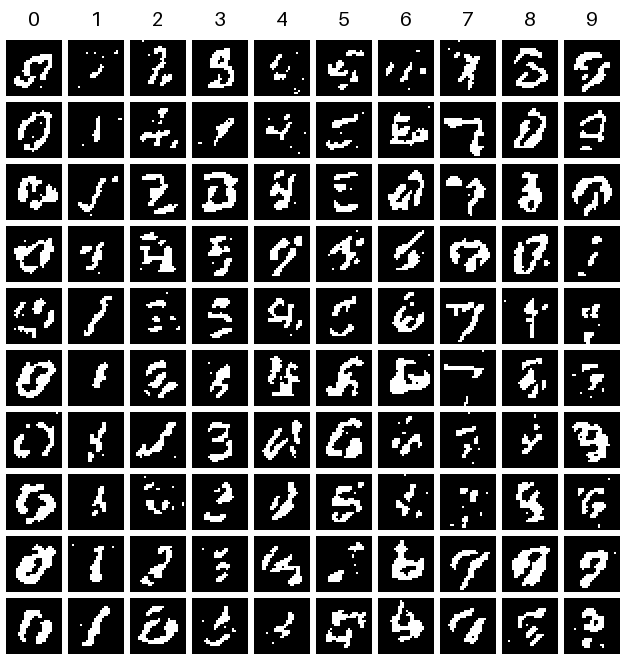
\includegraphics[width=\linewidth]{figures/digits_fvsbn.png}
  \caption{Samples grouped by predicted digit: columns $0\dots9$, ten draws per column.}
\end{subfigure}\hfill
\begin{subfigure}{0.40\textwidth}
  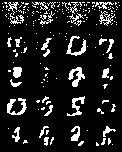
\includegraphics[width=\linewidth]{figures/fvsbn_progress.png}
  \caption{Training stages 1, 101, 201, 301 and 400 (one stage per row).}
\end{subfigure}

\vspace{2pt}
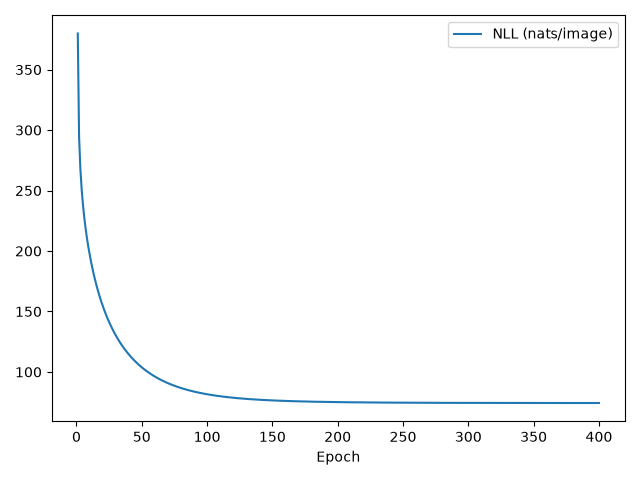
\includegraphics[width=0.52\linewidth]{figures/fvsbn_loss.png}
\caption{FVSBN: samples, training progress and training negative log-likelihood.}
\label{fig:fvsbn}
\end{figure}

\begin{figure}[H]
\centering
\begin{subfigure}{0.46\textwidth}
  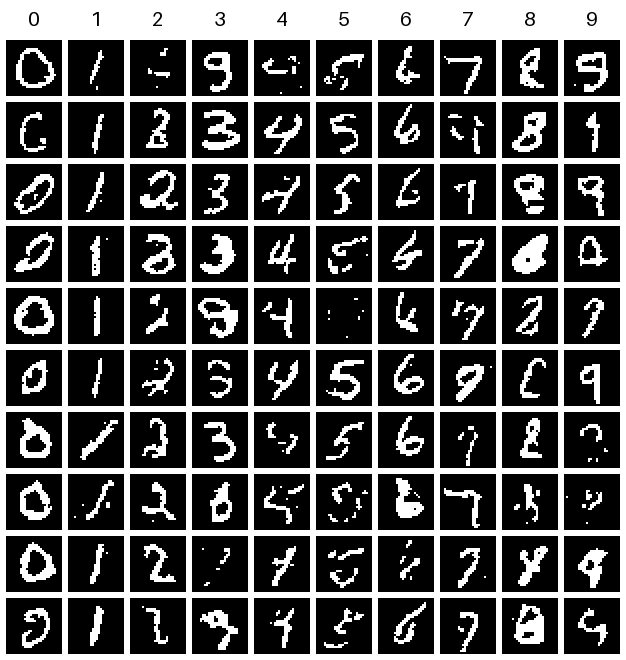
\includegraphics[width=\linewidth]{figures/digits_made.png}
  \caption{Samples grouped by predicted digit, same layout as Figure~\ref{fig:fvsbn}.}
\end{subfigure}\hfill
\begin{subfigure}{0.40\textwidth}
  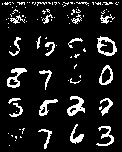
\includegraphics[width=\linewidth]{figures/made_progress.png}
  \caption{Training stages, same rows as Figure~\ref{fig:fvsbn}.}
\end{subfigure}

\vspace{2pt}
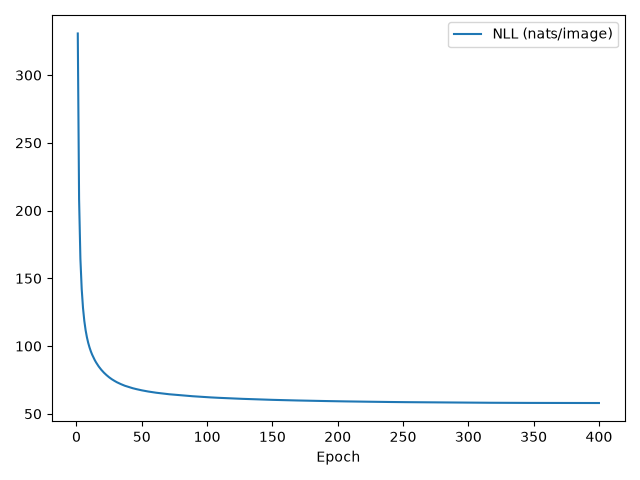
\includegraphics[width=0.52\linewidth]{figures/made_loss.png}
\caption{MADE: samples, training progress and training negative log-likelihood.}
\label{fig:made}
\end{figure}

\begin{figure}[H]
\centering
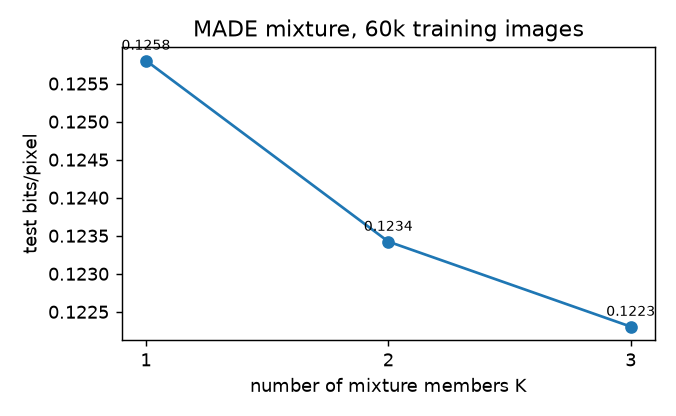
\includegraphics[width=0.52\linewidth]{figures/ensemble_ablation.png}
\caption{Test bits per pixel of the MADE mixture as a function of the number of members $K$
on the same $10{,}000$ test images.}
\label{fig:ensemble}
\end{figure}

\subsection{Adversarial models}
\label{sec:gan-results}

\begin{table}[H]
\centering
\caption{Generative adversarial models, scored with an independent classifier. Confidence and
entropy are computed from $2{,}000$ samples; FD is a feature Fr\'echet distance to $5{,}000$
real images (lower is better). Real MNIST: $0.939$ / $2.299$ / $0$.}
\label{tab:gan}
\small
\begin{tabular}{llrrrrr}
\toprule
Model & Architecture & Epochs & Confidence & Entropy & FD & s/epoch \\
\midrule
MLP, initial run & fully connected & 60 & 0.8802 & 2.1737 & 34.61 & 5.29 \\
MLP, shared learning rate & fully connected & 150 & 0.8787 & 2.1655 & 38.30 & 0.89 \\
MLP, two-timescale & fully connected & 150 & \textbf{0.8852} & 2.2808 & 7.71 & 0.90 \\
DCGAN, live weights & convolutional & 400 & 0.8477 & 2.2735 & 7.15 & 0.80 \\
DCGAN, moving average & convolutional & 400 & 0.8476 & 2.2740 & \textbf{7.12} & 0.80 \\
\bottomrule
\end{tabular}
\end{table}

Figure~\ref{fig:mlp} shows the fully connected baseline and Figure~\ref{fig:dcgan} the
convolutional model; the appendix compares the three fully connected runs side by side.
The first row of Table~\ref{tab:gan} is an initial run with a single learning rate at a batch
size of $128$. Increasing the batch while keeping that rate made the discriminator dominant
and raised the feature distance to $38.30$, which is the empirical reason for adopting the
two-timescale rule. With the rule, the same architecture reaches
$7.71$, and the convolutional architecture reaches $7.15$ with visibly smoother strokes.

All five runs cover the ten digits, contain no blank images and produce class histograms
without a dominant class, so there is no complete mode collapse. The smallest predicted-class
share in $2{,}000$ samples is $3.5\%$ for the initial run and $6.2\%$ for the convolutional
one, while the largest is $19.3\%$ and $15.5\%$ respectively, so coverage is uneven rather
than absent: 9 and 8 are drawn more often than 4 and 5, and the gap is visible in the digit
columns of Figures~\ref{fig:mlp}--\ref{fig:dcgan}.

The generator and discriminator losses of the convolutional run stay in a narrow band --- about
$0.93$ and $1.12$ at the end of training --- which is the oscillation expected around the
adversarial equilibrium rather than evidence of convergence; the loss panel of
Figure~\ref{fig:dcgan} shows the same behaviour over all 400 epochs.

Using the moving average changes the checkpoint only; the training curve and the loss values
are identical to the live-weight run. The three external statistics are also almost identical:
confidence $0.8476$ against $0.8477$, entropy $2.2740$ against $2.2735$, and
$\mathrm{FD}=7.12$ against $7.15$. A difference of $0.03$ is far below the run-to-run spread of
this architecture, since two runs of the same configuration differ by $0.14$ in FD
($7.15$ and $7.29$ for two such runs) because cuDNN convolution kernels are not
bit-reproducible. The moving average is therefore reported as a stabilising option that costs
nothing at inference, not as a demonstrated quality gain; the sample grid is included so the
reader can judge the visual difference independently.

\begin{figure}[H]
\centering
\begin{subfigure}{0.46\textwidth}
  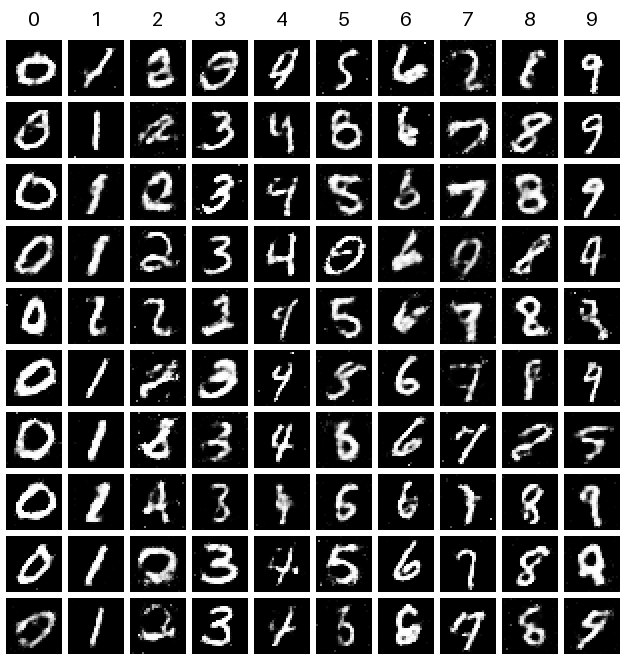
\includegraphics[width=\linewidth]{figures/digits_mlp.png}
  \caption{Samples grouped by predicted digit.}
\end{subfigure}\hfill
\begin{subfigure}{0.40\textwidth}
  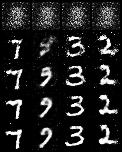
\includegraphics[width=\linewidth]{figures/mlp_progress.png}
  \caption{Training stages with four fixed latent vectors per row.}
\end{subfigure}

\vspace{2pt}
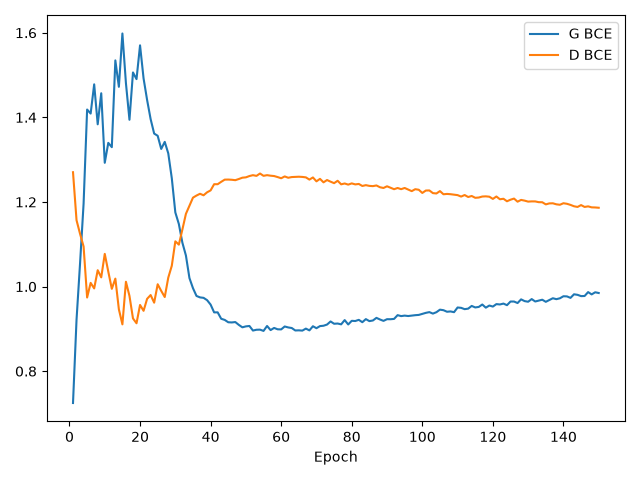
\includegraphics[width=0.52\linewidth]{figures/mlp_loss.png}
\caption{Fully connected baseline trained with the two-timescale rule.}
\label{fig:mlp}
\end{figure}

\begin{figure}[H]
\centering
\begin{subfigure}{0.46\textwidth}
  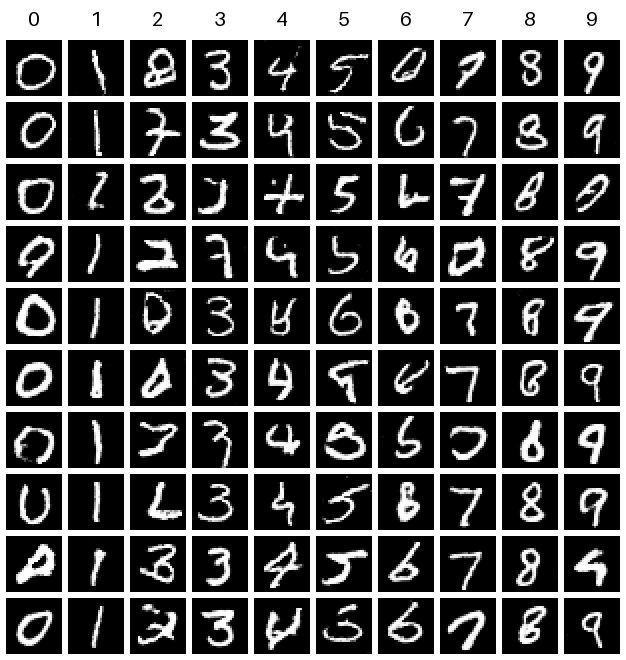
\includegraphics[width=\linewidth]{figures/digits_dcgan_raw.png}
  \caption{Live weights.}
\end{subfigure}\hfill
\begin{subfigure}{0.46\textwidth}
  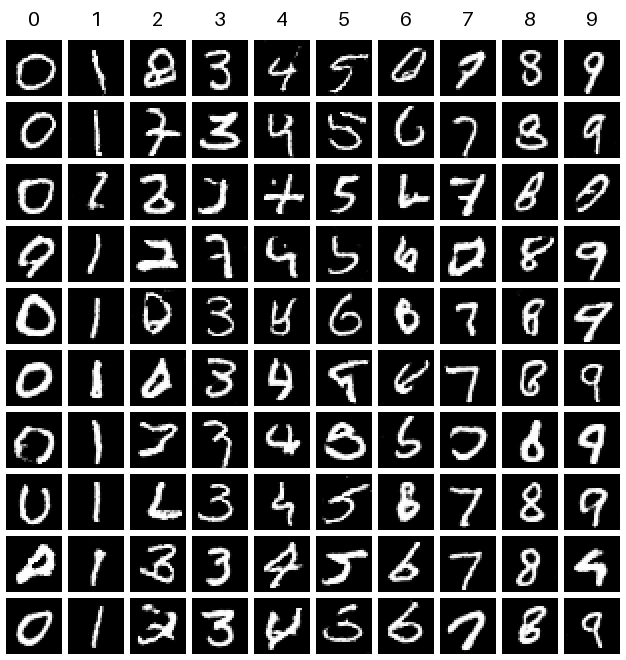
\includegraphics[width=\linewidth]{figures/digits_dcgan_ema.png}
  \caption{Moving average.}
\end{subfigure}

\vspace{2pt}
\begin{subfigure}{0.30\textwidth}
  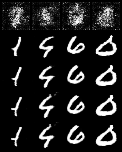
\includegraphics[width=\linewidth]{figures/dcgan_progress.png}
  \caption{Training stages.}
\end{subfigure}\hfill
\begin{subfigure}{0.45\textwidth}
  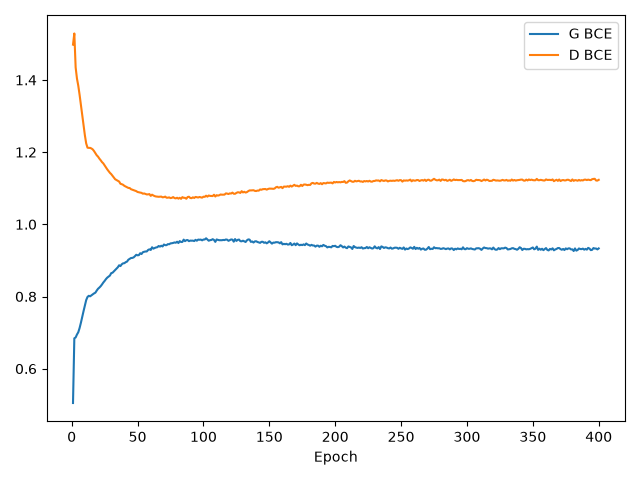
\includegraphics[width=\linewidth]{figures/dcgan_loss.png}
  \caption{Generator and discriminator loss.}
\end{subfigure}
\caption{Convolutional generator: samples grouped by predicted digit for the live weights and
for the moving average, the training-stage grid and the adversarial losses.}
\label{fig:dcgan}
\end{figure}

\subsection{Hyperparameter analysis}
\label{sec:hyper}

\begin{table}[H]
\centering
\caption{Masked autoregressive configurations. Selection used $5{,}000$ images held out of the
training split; the test column is shown only for reference and did not guide the choice.}
\label{tab:sweep}
\small
\begin{tabular}{lrrr}
\toprule
Configuration & Validation bpp & Test bpp & Train (s) \\
\midrule
1536 units, 1 layer, 400 epochs & \textbf{0.1287} & 0.1266 & 44 \\
2048 units, 1 layer, 400 epochs & 0.1295 & 0.1276 & 44 \\
1024 units, 1 layer, 400 epochs & 0.1320 & 0.1296 & 69 \\
1024 units, 1 layer, 800 epochs & 0.1341 & 0.1318 & 86 \\
1024 units, 2 layers, weight decay $10^{-3}$ & 0.1376 & 0.1349 & 64 \\
1024 units, 2 layers, 400 epochs & 0.1443 & 0.1416 & 47 \\
1024 units, 2 layers, weight decay $10^{-2}$ & 0.1450 & 0.1419 & 75 \\
1024 units, 2 layers, dropout $0.1$ & 0.1469 & 0.1438 & 49 \\
512 units, 1 layer, 400 epochs & 0.1618 & 0.1589 & 45 \\
\bottomrule
\end{tabular}
\end{table}

Table~\ref{tab:sweep} reports the nine most informative of fourteen configurations that were
trained for this study. Three findings shaped the final model.

A single wide layer is consistently better than two narrower ones: at $1024$ units the
validation cost is $0.1320$ against $0.1443$ bits per pixel. With the mask conditions of
Equation~\ref{eq:made-masks}, every additional masked layer restricts the set of admissible
paths, so depth buys little here and costs optimisation difficulty.
Dropout and weight decay did not help at this data size, which suggests that the gap between
training and test likelihood is not the binding constraint.
Doubling the number of epochs from $400$ to $800$ made the validation cost worse
($0.1320 \to 0.1341$), so the cosine schedule at $400$ epochs was kept.

\subsection{Per-digit showcase}
\label{sec:digits}

\begin{figure}[H]
\centering
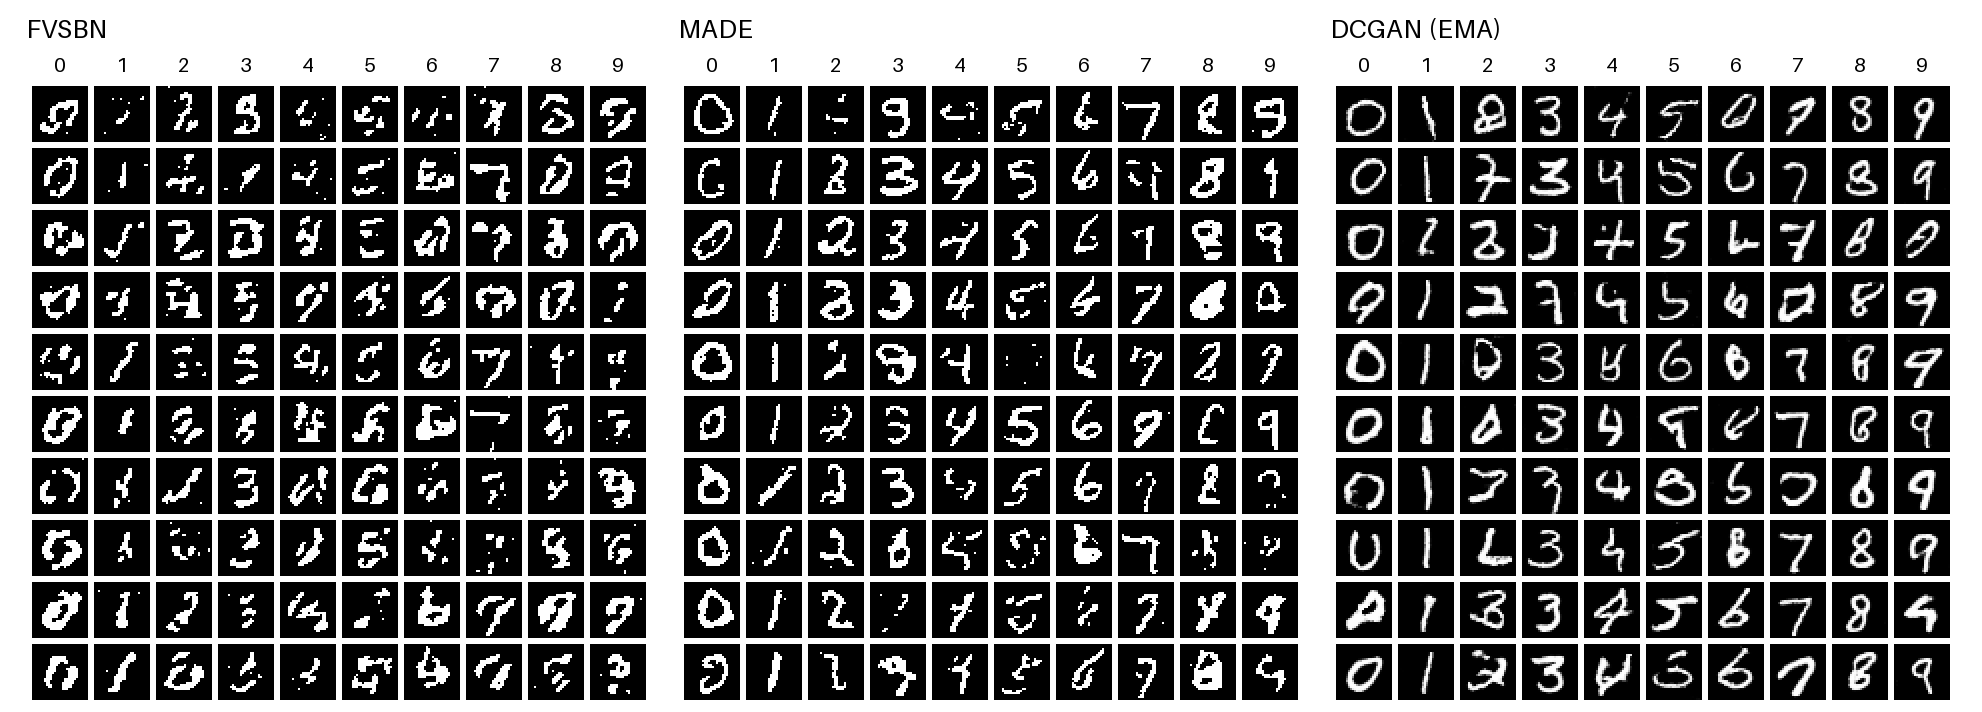
\includegraphics[width=\linewidth]{figures/digit_grid.png}
\caption{Unconditional samples grouped by the digit predicted by the independent classifier,
shown side by side for the linear model, the masked autoregressive model and the convolutional
generator. Columns are $0,1,\dots,9$; each row is an independent draw. The same convention is
used in Figures~\ref{fig:fvsbn}--\ref{fig:dcgan}.}
\label{fig:digits}
\end{figure}

The generators are unconditional and have no class input, so a digit-ordered grid cannot be
produced by conditioning. As described in Section~\ref{sec:metrics}, $4{,}000$ unconditional
samples are drawn per model, labelled by the classifier, and the first ten assigned to each
digit are kept; samples are not ranked by confidence and are not selected for appearance.
The pool size is reported because it shows that the selection does not hide a collapse: the
rarest predicted class contains $52$ of $4{,}000$ draws for the linear model but $249$ for
MADE and $243$ for the convolutional generator with the moving average.

\subsection{Run time}

Training and sampling times are listed in Table~\ref{tab:ar} for the autoregressive models and
Table~\ref{tab:gan} for the adversarial ones. The full pipeline on one RTX~5080 laptop GPU
--- three mixture members at $60{,}000$ images, their $10{,}000$-image counterparts, one
adversarial model, sampling, evaluation and the digit grid --- takes about ten minutes, of
which the adversarial model accounts for roughly $60\%$.
Autoregressive sampling is the slowest inference path because it performs $784$ sequential
forward passes, but a batch of $100$ images still completes in about $0.1$~s.

%----------------------------------------------------------------------------------------
\section{Discussion}
\label{sec:discussion}
%----------------------------------------------------------------------------------------

\paragraph{Resolution.}
The $14\times14$ ablation shows why bits per pixel is the right unit. The $14\times14$ model reaches $33.66$ nats per image, the $28\times28$ model
$68.45$; the first looks better until the pixel count is accounted for, at which point the
full-resolution model is twice as efficient per pixel. The apparent paradox comes from
area-downsampling: averaging four pixels and thresholding produces a denser, less predictable
binary image, so each coarse pixel carries more entropy than each fine pixel.

\paragraph{Linear versus nonlinear.}
At $28\times28$ the linear model is only $9.5\%$ worse than the masked network, while at
$14\times14$ the gap was $17\%$. The nonlinear model therefore helps most where the binary
resolution destroys information; at full resolution a large part of the remaining structure is
still additive. This also explains why the mixture, rather than a larger network, was the
cheapest way to improve the likelihood: widening from $1536$ to $2048$ units did nothing,
while averaging three independently trained models removed $2$ nats.

\paragraph{Adversarial stability.}
The three adversarial runs illustrate the interaction between batch size and learning rate.
The initial run used $128$-image batches with a shared rate and converged slowly but stably.
Moving to $512$-image batches without changing the rate reduced the noise in the discriminator
gradient enough for it to dominate, and the measured distribution distance degraded beyond the
initial run. Halving the discriminator rate restored balance, and the convolutional architecture
then improved the distance further while producing smoother strokes. The moving average is a
cheap additional stabiliser: it does not change training, only which weights are used at
sampling time.
Class histograms show no collapse, but the imbalance between frequent (9, 8) and rare (4, 5)
shapes persists in every run, so coverage is uneven rather than absent.

\paragraph{Limitations.}
All results are single-seed except the autoregressive mixture, so no significance test is
offered for the adversarial comparisons; the mixture spread ($\pm0.08$ nats) is reported as a
rough guide to seed noise. The Fr\'echet distance uses a classifier trained on MNIST rather
than an external feature extractor, so it is a proxy and is treated as such. The binarisation
threshold is fixed at $0.5$; the dynamically binarised variant used in some of the literature
is harder, and numbers should not be compared across the two protocols. Finally, all models
are unconditional, so the digit grid of Section~\ref{sec:digits} is a selection rather than a
demonstration of conditional control.

%----------------------------------------------------------------------------------------
\section{Conclusion}
%----------------------------------------------------------------------------------------

The three required generators were implemented, trained and evaluated with the metric that
each formulation supports. On $28\times28$ binarised digits the linear fully visible model
reaches $0.1393$ bits per pixel and the masked autoregressive model $0.1260$; mixing three
independently seeded members lowers this to $0.1223$ at three times the parameter count. On
the original grayscale digits the convolutional generator reaches a feature distance of
$7.12$, against $34.61$ for the fully connected initial run, with ten classes covered and no
blank samples. The accompanying repository contains all checkpoints, per-run configurations,
training histories, the scripts that reproduce every table and figure, and a single command
that reruns the pipeline on a Windows machine with a CUDA GPU.

\newpage
\appendix

%----------------------------------------------------------------------------------------
\section{Run instructions}
%----------------------------------------------------------------------------------------

The repository is self-contained: MNIST is read from the bundled \texttt{data/} folder, and no
network access is needed. On Windows with the prepared virtual environment:

\begin{verbatim}
$py = 'D:\HKStudy\.venv\Scripts\python.exe'
& $py -m cs5494.checks units
& $py -m cs5494.train --models fvsbn made --samples 60000 --test-samples 10000 `
      --side 28 --hidden 1536 --layers 1 --epochs 400 --batch 1024 --lr 0.001 `
      --scheduler cosine --device cuda --workers 4 --seed 42 `
      --output results/autoregressive
& $py -m cs5494.train --models gan --samples 60000 --epochs 400 --batch 512 `
      --lr 0.0002 --lr-d 0.00002 --arch dcgan --scheduler cosine --ema 0.999 `
      --device cuda --workers 4 --output results/gan_ema
& $py -m cs5494.evaluate mixture --runs results/made_seed42 `
      results/made_seed43 results/made_seed44
& $py -m cs5494.evaluate gan --runs results/gan_ema --weights ema
& $py -m cs5494.figures digits
& $py -m cs5494.checks report
cd report; powershell -NoProfile -ExecutionPolicy Bypass -File build.ps1
\end{verbatim}

The same commands work on Colab after installing \texttt{requirements.txt} and replacing
the interpreter with \texttt{python}; \texttt{assignment.ipynb} wraps them in a notebook.
The script \texttt{run\_windows.ps1} runs the whole pipeline, including the checks and
the comparison document. Every script comments the non-obvious parts, and each run writes a
\texttt{config.json} that records the exact arguments, so any table entry can be traced back
to the command that produced it.

%----------------------------------------------------------------------------------------
\section{Code map and additional figures}
%----------------------------------------------------------------------------------------

\begin{table}[H]
\centering
\caption{Files in the shared folder.}
\small
\begin{tabular}{ll}
\toprule
File & Responsibility \\
\midrule
\texttt{cs5494/train.py} & models (FVSBN, MADE, MLP/DCGAN), training loop, previews, metrics \\
\texttt{cs5494/sample.py} & resample from a checkpoint, optionally the moving-average weights \\
\texttt{cs5494/evaluate.py} & classifier scores for GANs, mixture likelihood for MADE \\
\texttt{cs5494/figures.py} & per-digit grids and the MLP training-regime figure \\
\texttt{cs5494/checks.py} & unit tests, NLL re-computation, report/JSON consistency, hashes \\
\texttt{cs5494/compare\_runs.py} & side-by-side comparison of result folders \\
\texttt{report/source\_code\_appendix.tex} & verbatim source of all eight modules (Appendix~C) \\
\texttt{report/} & this document, \texttt{main.tex} + \texttt{refs.bib} \\
\bottomrule
\end{tabular}
\end{table}

\begin{figure}[H]
\centering
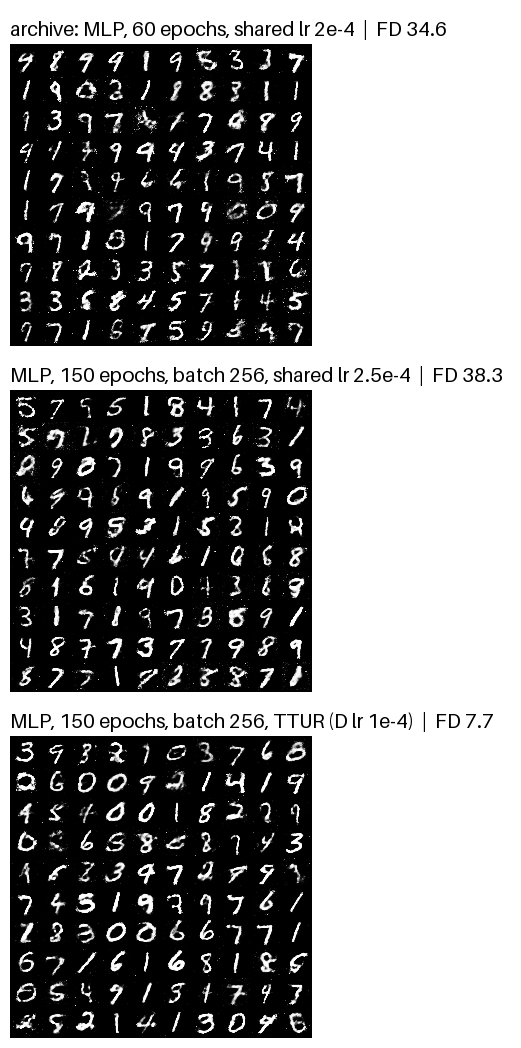
\includegraphics[width=0.62\linewidth]{figures/mlp_variants.png}
\caption{Fully connected generator under three training regimes. The first uses a
shared learning rate, the second keeps that rate at a larger batch, and the third applies the
two-timescale rule. Feature distances are $34.61$, $38.30$ and $7.71$ respectively.}
\label{fig:mlp-variants}
\end{figure}

% ---------------------------------------------------------------------------------------
% Appendix C: complete source code.
% Generated from cs5494/ at packaging time. This is a snapshot: if the Python files are
% edited afterwards, re-run the generator or delete this appendix. Long lines are folded by
% the listings package for printing only; the authoritative copies are cs5494/*.py.
% ---------------------------------------------------------------------------------------

\newpage
\section{Complete source code}
\label{app:code}

The shared folder contains the runnable package \texttt{cs5494/}. Appendix~A lists the
commands that reproduce every table and figure, and Appendix~B maps each file to its
responsibility. This appendix reproduces all eight modules verbatim so that the submitted
report is self-contained even before a public code link is available. A single typographic
dash in \texttt{compare\_runs.py} is printed as an ASCII hyphen; no executable statement is
affected. Line breaks inserted by the typesetting of long source lines are visual only.

\subsection*{cs5494/\_\_init\_\_.py --- package exports and version note}
\begin{lstlisting}
"""CS5494 assignment code: models, training, evaluation and figure generation.

Modules
    train.py          model definitions (FVSBN, MADE, MLP/DCGAN) and the training loop
    sample.py         draw samples from a saved checkpoint (GAN: live or EMA weights)
    evaluate.py       external scoring: classifier statistics for GANs, mixture likelihood
    figures.py        report figures: per-digit grids, MLP variant comparison
    checks.py         unit tests, NLL re-computation, report/JSON consistency, hashes
    compare_runs.py   side-by-side comparison of result folders
    sweep_made.py     hyper-parameter sweep for the masked autoregressive model

Run everything from the repository root, e.g.

    python -m cs5494.train --models fvsbn made --samples 60000 --side 28 --hidden 1536 ...
    python -m cs5494.evaluate gan --runs results/gan_ema --weights ema
    python -m cs5494.checks report
"""
\end{lstlisting}

\subsection*{cs5494/train.py --- FVSBN, MADE, MLP-GAN, DCGAN and the training loop}
\begin{lstlisting}
"""CS5494: FVSBN, neural autoregressive MADE, and GAN on MNIST."""
import argparse, json, random, time
from pathlib import Path
import numpy as np
import torch
from torch import nn
from torch.nn import functional as F
from torch.utils.data import DataLoader, TensorDataset
from torchvision.datasets import MNIST
from torchvision import transforms
from torchvision.utils import save_image
import matplotlib
matplotlib.use('Agg')
import matplotlib.pyplot as plt

class MaskedLinear(nn.Linear):
    def __init__(self, ni, no, mask):
        super().__init__(ni, no)
        self.register_buffer('mask', mask.float())
    def forward(self, x):
        return F.linear(x, self.weight * self.mask, self.bias)

class Autoregressive(nn.Module):
    def __init__(self, dim, hidden=0, layers=1, dropout=0.0):
        super().__init__()
        self.dim = dim
        # Output i can only see pixels j < i; never the current/future pixel.
        degrees = torch.arange(dim)
        if hidden:
            # MADE ordering: hidden degree cycles over 0..dim-2. Every edge keeps the
            # hidden degree >= its input degree, and the output edge is strictly greater,
            # so no path can carry information from pixel i or later into output i.
            h = torch.arange(hidden) % (dim - 1)
            seq = [MaskedLinear(dim, hidden, h[:,None] >= degrees[None,:]), nn.ReLU()]
            if dropout > 0: seq.append(nn.Dropout(dropout))
            for _ in range(max(1, layers) - 1):
                seq += [MaskedLinear(hidden, hidden, h[:,None] >= h[None,:]), nn.ReLU()]
                if dropout > 0: seq.append(nn.Dropout(dropout))
            seq += [MaskedLinear(hidden, dim, degrees[:,None] > h[None,:])]
            self.net = nn.Sequential(*seq)
        else:
            self.net = MaskedLinear(dim, dim, degrees[:,None] > degrees[None,:])
    def forward(self, x):
        return self.net(x)
    @torch.no_grad()
    def sample(self, n, device):
        x = torch.zeros(n, self.dim, device=device)
        for i in range(self.dim):
            x[:,i] = torch.bernoulli(self(x)[:,i].sigmoid())
        return x

class Generator(nn.Module):
    def __init__(self):
        super().__init__()
        self.net = nn.Sequential(nn.Linear(64,256),nn.LeakyReLU(.2),nn.Linear(256,512),nn.LeakyReLU(.2),nn.Linear(512,784),nn.Tanh())
    def forward(self, z): return self.net(z)

class Discriminator(nn.Module):
    def __init__(self):
        super().__init__()
        self.net = nn.Sequential(nn.Linear(784,512),nn.LeakyReLU(.2),nn.Linear(512,256),nn.LeakyReLU(.2),nn.Linear(256,1))
    def forward(self, x): return self.net(x).flatten()

class DCGenerator(nn.Module):
    """DCGAN generator, 64 -> 7x7 -> 14x14 -> 28x28, returned flattened like the MLP one."""
    def __init__(self):
        super().__init__()
        self.net = nn.Sequential(
            nn.Linear(64,128*7*7), nn.Unflatten(1,(128,7,7)), nn.BatchNorm2d(128), nn.ReLU(True),
            nn.ConvTranspose2d(128,64,4,2,1), nn.BatchNorm2d(64), nn.ReLU(True),
            nn.ConvTranspose2d(64,1,4,2,1), nn.Tanh(), nn.Flatten(1))
    def forward(self, z): return self.net(z)

class DCDiscriminator(nn.Module):
    def __init__(self):
        super().__init__()
        self.net = nn.Sequential(
            nn.Unflatten(1,(1,28,28)),
            nn.Conv2d(1,64,4,2,1), nn.LeakyReLU(.2),
            nn.Conv2d(64,128,4,2,1), nn.BatchNorm2d(128), nn.LeakyReLU(.2),
            nn.Flatten(1), nn.Linear(128*7*7,1))
    def forward(self, x): return self.net(x).flatten()

def build_gan(arch):
    if arch == 'dcgan':
        return DCGenerator(), DCDiscriminator()
    return Generator(), Discriminator()

def run(a):
    random.seed(a.seed); np.random.seed(a.seed); torch.manual_seed(a.seed)
    device = torch.device(a.device if a.device != 'auto' else ('cuda' if torch.cuda.is_available() else 'mps' if torch.backends.mps.is_available() else 'cpu'))
    if device.type=='cuda':
        # Fixed-size layers: benchmark off, but allow TF32 matmuls on Ampere+ for speed.
        torch.backends.cuda.matmul.allow_tf32 = bool(a.tf32)
        torch.backends.cudnn.allow_tf32 = bool(a.tf32)
    out = Path(a.output); out.mkdir(parents=True, exist_ok=True)
    (out/'config.json').write_text(json.dumps(vars(a)|{'resolved_device':str(device),'device_name':torch.cuda.get_device_name(0) if device.type=='cuda' else str(device)},indent=2))
    train = MNIST(a.data,train=True,download=True,transform=transforms.ToTensor())
    test = MNIST(a.data,train=False,download=True,transform=transforms.ToTensor())
    indices = torch.randperm(len(train))[:a.samples]
    torch.save(indices,out/'training_indices.pt')
    raw = train.data[indices].float().unsqueeze(1)/255
    test_raw = test.data[:a.test_samples].float().unsqueeze(1)/255
    metrics = {}
    for name in a.models:
        folder=out/name; folder.mkdir(exist_ok=True)
        gan = name == 'gan'; side=28 if gan else a.side
        x = raw.flatten(1)*2-1 if gan else (F.interpolate(raw,size=(side,side),mode='area')>=.5).float().flatten(1)
        # Optional held-out split used only for hyperparameter selection (never for gradients).
        if not gan and a.val > 0:
            xval, xtr = x[:a.val], x[a.val:]
        else:
            xval, xtr = None, x
        loader=DataLoader(TensorDataset(xtr),batch_size=a.batch,shuffle=True,num_workers=a.workers,
                          pin_memory=device.type=='cuda',persistent_workers=a.workers>0)
        if gan:
            gen, discr = build_gan(a.arch)
            model = gen.to(device); disc = discr.to(device)
            opt = torch.optim.Adam(model.parameters(), lr=a.lr, betas=(.5,.999))
            dop=torch.optim.Adam(disc.parameters(),lr=a.lr_d if a.lr_d else a.lr,betas=(.5,.999))
            fixed=torch.randn(20,64,device=device)
            # Exponential moving average of the generator parameters. Buffers such as
            # BatchNorm running statistics are copied from the live model at save time.
            ema = ({k: v.detach().clone() for k, v in model.named_parameters()}
                   if a.ema > 0 else None)
        else:
            model=Autoregressive(side*side, a.hidden if name=='made' else 0,
                                 a.layers if name=='made' else 1,
                                 a.dropout if name=='made' else 0.0).to(device)
            opt=torch.optim.Adam(model.parameters(),lr=a.lr,betas=(.9,.999),weight_decay=a.weight_decay)
        sched=(torch.optim.lr_scheduler.CosineAnnealingLR(opt,T_max=a.epochs,eta_min=a.lr*.02)
               if a.scheduler=='cosine' else None)
        dsched=(torch.optim.lr_scheduler.CosineAnnealingLR(dop,T_max=a.epochs,eta_min=(a.lr_d or a.lr)*.02)
                if gan and a.scheduler=='cosine' else None)
        history=[]; snapshots=[]; start=time.perf_counter()
        for epoch in range(a.epochs):
            e0=time.perf_counter()
            total=0.; dtotal=0.; count=0
            for (batch,) in loader:
                batch=batch.to(device,non_blocking=True); n=len(batch)
                if gan:
                    dop.zero_grad(); fake=model(torch.randn(n,64,device=device)).detach()
                    dl=F.binary_cross_entropy_with_logits(disc(batch),torch.ones(n,device=device))+F.binary_cross_entropy_with_logits(disc(fake),torch.zeros(n,device=device))
                    dl.backward(); dop.step(); dtotal+=dl.item()*n
                    disc.requires_grad_(False)
                    opt.zero_grad(); loss=F.binary_cross_entropy_with_logits(disc(model(torch.randn(n,64,device=device))),torch.ones(n,device=device))
                    loss.backward(); opt.step(); disc.requires_grad_(True)
                    if ema is not None:
                        with torch.no_grad():
                            for k, p in model.named_parameters():
                                ema[k].mul_(a.ema).add_(p, alpha=1-a.ema)
                else:
                    opt.zero_grad(); loss=F.binary_cross_entropy_with_logits(model(batch),batch,reduction='none').sum(1).mean()
                    loss.backward(); opt.step()
                total+=loss.item()*n; count+=n
            row={'epoch':epoch+1,'loss':total/count,'seconds':time.perf_counter()-e0}
            if gan: row['discriminator_loss']=dtotal/count
            history.append(row); print(name,{k:(round(v,4) if isinstance(v,float) else v) for k,v in row.items()},flush=True)
            if sched: sched.step()
            if dsched: dsched.step()
            if epoch in {0,a.epochs//4,a.epochs//2,3*a.epochs//4,a.epochs-1}:
                model.eval()
                with torch.no_grad(): samples=(model(fixed)+1)/2 if gan else model.sample(20,device)
                model.train()
                images=samples.cpu().reshape(-1,1,side,side); save_image(images,folder/f'epoch_{epoch+1:03}.png',nrow=5); snapshots.append(images[:4])
        if device.type=='mps': torch.mps.synchronize()
        if device.type=='cuda': torch.cuda.synchronize()
        elapsed=time.perf_counter()-start
        model.eval()
        inference_start=time.perf_counter()
        with torch.no_grad(): samples=(model(torch.randn(100,64,device=device))+1)/2 if gan else model.sample(100,device)
        images=samples.cpu().reshape(-1,1,side,side)
        infer=time.perf_counter()-inference_start
        save_image(images,folder/'samples.png',nrow=10)
        save_image(torch.cat(snapshots),folder/'progress.png',nrow=4)
        torch.save(model.state_dict(),folder/'model.pt')
        if gan:
            torch.save(disc.state_dict(),folder/'discriminator.pt')
            if ema is not None:
                sd = {k: v.clone() for k, v in model.state_dict().items()}
                for k, v in ema.items():
                    sd[k] = v.clone()
                torch.save(sd, folder/'model_ema.pt')
        result={'training_and_preview_seconds':elapsed,'inference_100_seconds':infer,'training_samples':len(xtr)}
        if gan and ema is not None:
            result['ema_decay'] = a.ema
        if not gan:
            def _nll(batch_x):
                with torch.no_grad():
                    return sum(F.binary_cross_entropy_with_logits(model(b.to(device)),b.to(device),reduction='sum').item()
                               for b in batch_x.split(a.batch))/len(batch_x)
            tx=(F.interpolate(test_raw,size=(side,side),mode='area')>=.5).float().flatten(1)
            nll=_nll(tx)
            result|={'test_nll_nats_per_image':nll,'test_bits_per_pixel':nll/(side*side*np.log(2))}
            if xval is not None:
                vnll=_nll(xval)
                result|={'validation_samples':len(xval),'validation_nll_nats_per_image':vnll,
                         'validation_bits_per_pixel':vnll/(side*side*np.log(2))}
        metrics[name]=result
        print(name,'summary',{k:round(v,4) for k,v in result.items()},flush=True)
        (folder/'history.json').write_text(json.dumps(history,indent=2))
        plt.figure(); plt.plot([r['epoch'] for r in history],[r['loss'] for r in history],label='G BCE' if gan else 'NLL (nats/image)')
        if gan: plt.plot([r['epoch'] for r in history],[r['discriminator_loss'] for r in history],label='D BCE')
        plt.xlabel('Epoch'); plt.legend(); plt.tight_layout(); plt.savefig(folder/'loss.png'); plt.close()
        (out/'metrics.json').write_text(json.dumps(metrics,indent=2))

if __name__=='__main__':
    p=argparse.ArgumentParser()
    p.add_argument('--models',nargs='+',choices=['fvsbn','made','gan'],default=['fvsbn','made','gan'])
    p.add_argument('--data',default='data'); p.add_argument('--output',default='outputs/main')
    p.add_argument('--samples',type=int,default=20000); p.add_argument('--test-samples',type=int,default=2000)
    p.add_argument('--epochs',type=int,default=20); p.add_argument('--batch',type=int,default=128)
    p.add_argument('--side',type=int,default=14); p.add_argument('--hidden',type=int,default=512)
    p.add_argument('--layers',type=int,default=1,help='masked hidden layers for MADE')
    p.add_argument('--dropout',type=float,default=0.0,help='dropout on MADE hidden activations')
    p.add_argument('--weight-decay',dest='weight_decay',type=float,default=0.0)
    p.add_argument('--val',type=int,default=0,help='leading samples held out as validation (autoregressive only)')
    p.add_argument('--arch',choices=['mlp','dcgan'],default='mlp',help='GAN generator/discriminator architecture')
    p.add_argument('--scheduler',choices=['none','cosine'],default='none')
    p.add_argument('--ema',type=float,default=0.0,
                   help='decay for an exponential moving average of the GAN generator (0 disables)')
    p.add_argument('--lr',type=float,default=.0002); p.add_argument('--seed',type=int,default=42); p.add_argument('--device',default='auto')
    p.add_argument('--lr-d',dest='lr_d',type=float,default=0.0,
                   help='optional discriminator learning rate (TTUR); 0 keeps --lr')
    p.add_argument('--workers',type=int,default=0)
    p.add_argument('--tf32',type=int,default=1,choices=[0,1])
    a=p.parse_args()
    if not (2<=a.side<=28 and a.samples>0 and a.test_samples>0 and a.epochs>0 and a.batch>0): p.error('invalid dimensions or counts')
    run(a)
\end{lstlisting}

\subsection*{cs5494/sample.py --- draw samples from a saved checkpoint}
\begin{lstlisting}
"""Generate samples from a saved run without retraining.

Reads the architecture back from the run's config.json, so MLP and DCGAN checkpoints
both work, as do linear FVSBNs and multi-layer MADE models.
"""
import argparse,json
from pathlib import Path
import torch
from cs5494.train import Autoregressive, build_gan
from torchvision.utils import save_image
p=argparse.ArgumentParser(); p.add_argument('run'); p.add_argument('model',choices=['fvsbn','made','gan']); p.add_argument('--seed',type=int,default=123); p.add_argument('--which',choices=['raw','ema'],default='raw',help='GAN only: use model_ema.pt'); a=p.parse_args()
r=Path(a.run); c=json.loads((r/'config.json').read_text()); torch.manual_seed(a.seed)
gan=a.model=='gan'; side=28 if gan else c['side']
if gan:
    m=build_gan(c.get('arch','mlp'))[0]
else:
    m=Autoregressive(side*side,c['hidden'] if a.model=='made' else 0,c.get('layers',1),c.get('dropout',0.0))
ckpt = r/a.model/(('model_ema.pt' if a.which=='ema' else 'model.pt') if gan else 'model.pt')
m.load_state_dict(torch.load(ckpt,map_location='cpu',weights_only=True)); m.eval()
n=64 if gan else 100
with torch.no_grad(): x=(m(torch.randn(n,64))+1)/2 if gan else m.sample(n,'cpu')
tag = 'samples_seed_%d%s.png' % (a.seed, '_ema' if (gan and a.which=='ema') else '')
save_image(x.reshape(-1,1,side,side),r/a.model/tag,nrow=10)
\end{lstlisting}

\subsection*{cs5494/evaluate.py --- independent classifier scores and mixture likelihood}
\begin{lstlisting}
"""External evaluation for the generative models.

Two sub-commands, both standardising their output as JSON next to the report:

    gan       trains (or loads) an independent MNIST classifier and scores every GAN
              checkpoint with confidence, class entropy and a feature Frechet distance.
    mixture   computes the held-out likelihood of a mixture of autoregressive models,
              p(x) = 1/K * sum_k p_k(x), for K = 1..n and writes the K-vs-bpp curve.

Examples
    python -m cs5494.evaluate gan --runs results/gan_ema --weights ema
    python -m cs5494.evaluate mixture --runs results/made_seed42 results/made_seed43 \
        results/made_seed44 --out results/ensemble_metrics.json
"""
import argparse, io, json, time
from pathlib import Path

import numpy as np
import torch
from torch import nn
from torch.nn import functional as F
from torchvision.datasets import MNIST

from cs5494.train import Autoregressive, build_gan


# --------------------------------------------------------------------------------------
# classifier used as an independent evaluator (also labels the per-digit figures)
# --------------------------------------------------------------------------------------
class Clf(nn.Module):
    def __init__(self):
        super().__init__()
        self.net = nn.Sequential(
            nn.Conv2d(1, 16, 3, padding=1), nn.ReLU(), nn.MaxPool2d(2),
            nn.Conv2d(16, 32, 3, padding=1), nn.ReLU(), nn.MaxPool2d(2),
            nn.Flatten(), nn.Linear(32*7*7, 128), nn.ReLU(), nn.Linear(128, 10))

    def forward(self, x):
        return self.net(x)

    def features(self, x):
        """128-d penultimate activations, used by the Frechet-distance proxy."""
        return self.net[:-2](x)


def load_classifier(path='comparisons/gan_classifier.pt', device='cpu'):
    clf = Clf()
    clf.load_state_dict(torch.load(path, map_location=device, weights_only=True))
    return clf.to(device).eval()


def train_or_load(args, dev):
    """Return an evaluated classifier, training it once if the cache is missing."""
    tr = MNIST('data', train=True, download=True)
    te = MNIST('data', train=False, download=True)
    xs = (tr.data.float()/255).unsqueeze(1)
    ys = tr.targets.clone()
    xt = (te.data.float()/255).unsqueeze(1).to(dev)
    yt = te.targets.clone().to(dev)

    clf = Clf().to(dev)
    ckpt = Path(args.classifier)
    if ckpt.exists():
        clf.load_state_dict(torch.load(ckpt, map_location=dev, weights_only=True))
        print('loaded cached classifier', ckpt)
    else:
        opt = torch.optim.Adam(clf.parameters(), 1e-3)
        n = min(args.train_n, len(xs))
        for ep in range(args.epochs):
            perm = torch.randperm(n)
            for i in range(0, n, 256):
                idx = perm[i:i+256]
                opt.zero_grad()
                F.cross_entropy(clf(xs[idx].to(dev)), ys[idx].to(dev)).backward()
                opt.step()
            with torch.no_grad():
                acc = (clf(xt).argmax(1) == yt).float().mean().item()
            print(f'classifier epoch {ep+1}: test acc {acc:.4f}')
        ckpt.parent.mkdir(parents=True, exist_ok=True)
        torch.save(clf.state_dict(), ckpt)
    clf.eval()
    return clf, xt, yt


def frechet(a, b):
    """Frechet distance between two feature Gaussians (the FID formula)."""
    from scipy.linalg import sqrtm
    mu1, mu2 = a.mean(0), b.mean(0)
    c1, c2 = np.cov(a, rowvar=False), np.cov(b, rowvar=False)
    covmean = sqrtm(c1 @ c2)
    if np.iscomplexobj(covmean):
        covmean = covmean.real
    return float(((mu1-mu2)**2).sum() + np.trace(c1 + c2 - 2*covmean))


# --------------------------------------------------------------------------------------
# gan: classifier statistics
# --------------------------------------------------------------------------------------
def cmd_gan(a):
    dev = torch.device('cuda' if torch.cuda.is_available() else 'cpu')
    torch.manual_seed(0)
    clf, xt, yt = train_or_load(a, dev)

    with torch.no_grad():
        acc = (clf(xt).argmax(1) == yt).float().mean().item()
        print(f'evaluator accuracy on 10,000 real test images: {acc:.4f}')
        p = clf(xt[:5000]).softmax(1)
        hist = torch.bincount(p.argmax(1), minlength=10).float()/len(p)
        ref = {'conf': p.max(1).values.mean().item(),
               'entropy': float(-(hist*torch.log(hist.clamp_min(1e-12))).sum()),
               'acc': acc}
        real_feat = clf.features(xt[:5000]).double().cpu().numpy()
    print('real MNIST reference:', {k: round(v, 4) for k, v in ref.items()})
    print(f'real self-FD (sanity, should be ~0): {frechet(real_feat, real_feat[500:]):.3f}')

    res = {'classifier_test_acc': acc, 'reference_real_mnist': ref, 'runs': {}}
    ckpt_name = 'model_ema.pt' if a.weights == 'ema' else 'model.pt'
    for run in a.runs:
        if not (Path(run)/'gan'/ckpt_name).exists():
            print('skip (no checkpoint):', run, ckpt_name)
            continue
        cfg = json.loads(io.open(Path(run)/'config.json', encoding='utf-8').read())
        g = build_gan(cfg.get('arch', 'mlp'))[0].to(dev)
        g.load_state_dict(torch.load(Path(run)/'gan'/ckpt_name, map_location=dev, weights_only=True))
        g.eval()
        key = run if a.weights == 'raw' else f'{run}::{a.weights}'
        torch.manual_seed(123)
        with torch.no_grad():
            imgs = (g(torch.randn(a.n, 64, device=dev))+1)/2
            imgs = imgs.clamp(0, 1).reshape(-1, 1, 28, 28)
            p = clf(imgs).softmax(1)
        hist = torch.bincount(p.argmax(1), minlength=10).float()/len(p)
        ent = float(-(hist*torch.log(hist.clamp_min(1e-12))).sum())
        with torch.no_grad():
            gen_feat = clf.features(imgs).double().cpu().numpy()
        fd = frechet(real_feat, gen_feat)
        row = {'conf': p.max(1).values.mean().item(), 'entropy': ent, 'fd': fd, 'acc': None,
               'classes_used': int((hist > 0.005).sum()),
               'class_hist': [round(float(v), 4) for v in hist],
               'blank_rate': float(((imgs.mean((1, 2, 3)) < .02) | (imgs.mean((1, 2, 3)) > .98)).float().mean())}
        res['runs'][key] = row
        print(f"{key:56s} conf={row['conf']:.4f} entropy={row['entropy']:.4f} "
              f"FD={fd:8.2f} classes={row['classes_used']:2d} blank={row['blank_rate']:.3f}")

    out = Path(a.out); out.parent.mkdir(parents=True, exist_ok=True)
    out.write_text(json.dumps(res, indent=2), encoding='utf-8')
    print('written', out)


# --------------------------------------------------------------------------------------
# mixture: likelihood of K autoregressive members
# --------------------------------------------------------------------------------------
def _load_member(run, device):
    run = Path(run)
    cfg = json.loads(io.open(run/'config.json', encoding='utf-8').read())
    side = cfg['side']
    model = Autoregressive(side*side, cfg['hidden'], cfg.get('layers', 1), cfg.get('dropout', 0.0))
    model.load_state_dict(torch.load(run/'made/model.pt', map_location=device, weights_only=True))
    return model.to(device).eval(), cfg, side


@torch.no_grad()
def _per_image_nll(model, x, device, batch=128):
    out = []
    for b in x.split(batch):
        b = b.to(device)
        out.append(F.binary_cross_entropy_with_logits(model(b), b, reduction='none').sum(1).cpu())
    return torch.cat(out)


def cmd_mixture(a):
    import matplotlib
    matplotlib.use('Agg')
    import matplotlib.pyplot as plt

    dev = torch.device('cuda' if torch.cuda.is_available() else 'cpu')
    models, cfgs, side = [], [], None
    for r in a.runs:
        m, cfg, s = _load_member(r, dev)
        models.append(m); cfgs.append(cfg); side = s

    test = MNIST('data', train=False, download=True)
    n = cfgs[0]['test_samples']
    raw = test.data[:n].float().unsqueeze(1)/255
    x = (F.interpolate(raw, size=(side, side), mode='area') >= .5).float().flatten(1)
    scale = side*side*np.log(2)

    members, nlls = [], []
    for run, m, cfg in zip(a.runs, models, cfgs):
        t0 = time.perf_counter()
        with torch.no_grad():
            m.sample(100, dev)
        infer = time.perf_counter()-t0
        p = _per_image_nll(m, x, dev)
        nlls.append(p)
        members.append({'run': str(run), 'seed': cfg.get('seed'),
                        'nats': float(p.mean()), 'bpp': float(p.mean()/scale),
                        'params': int(sum(q.numel() for q in m.parameters())),
                        'inference_100_seconds': infer})
        print(f"{str(run):34s} seed={cfg.get('seed')} nats={p.mean():.4f} bpp={p.mean()/scale:.4f}")

    metrics = {'side': side, 'test_samples': n, 'members': members, 'ensembles': []}
    plots = []
    for k in range(2, len(nlls)+1):
        mix = torch.logsumexp(-torch.stack(nlls[:k]), dim=0) - np.log(k)
        nats = float((-mix).mean())
        params = sum(m['params'] for m in members[:k])
        metrics['ensembles'].append({'k': k, 'members': [m['run'] for m in members[:k]],
                                     'nats': nats, 'bpp': nats/scale, 'params': params})
        print(f'mixture K={k}  nats={nats:.4f}  bpp={nats/scale:.4f}  params={params}')
        plots.append((k, nats/scale))
    plots.insert(0, (1, members[0]['bpp']))

    out = Path(a.out); out.parent.mkdir(parents=True, exist_ok=True)
    out.write_text(json.dumps(metrics, indent=2), encoding='utf-8')
    print('written', out)

    plt.figure(figsize=(5.2, 3.2))
    ks, bpps = zip(*plots)
    plt.plot(ks, bpps, 'o-')
    for k, b in plots:
        plt.annotate(f'{b:.4f}', (k, b), textcoords='offset points', xytext=(0, 6), ha='center', fontsize=8)
    plt.xticks(ks); plt.xlabel('number of mixture members K')
    plt.ylabel('test bits/pixel'); plt.title('MADE mixture, test split')
    plt.tight_layout()
    Path(a.figure).parent.mkdir(parents=True, exist_ok=True)
    plt.savefig(a.figure, dpi=130); plt.close()
    print('written', a.figure)


def main(argv=None):
    ap = argparse.ArgumentParser(description=__doc__, formatter_class=argparse.RawDescriptionHelpFormatter)
    sub = ap.add_subparsers(dest='cmd', required=True)

    g = sub.add_parser('gan', help='classifier statistics for GAN checkpoints')
    g.add_argument('--runs', nargs='+', default=['results/gan_initial', 'results/gan_mlp'])
    g.add_argument('--n', type=int, default=2000)
    g.add_argument('--weights', choices=['raw', 'ema'], default='raw')
    g.add_argument('--train-n', type=int, default=20000)
    g.add_argument('--epochs', type=int, default=3)
    g.add_argument('--classifier', default='comparisons/gan_classifier.pt')
    g.add_argument('--out', default='comparisons/gan_eval.json')
    g.set_defaults(func=cmd_gan)

    m = sub.add_parser('mixture', help='held-out likelihood of a mixture of MADE models')
    m.add_argument('--runs', nargs='+', required=True)
    m.add_argument('--out', default='results/ensemble_metrics.json')
    m.add_argument('--figure', default='results/ensemble_ablation.png')
    m.set_defaults(func=cmd_mixture)

    a = ap.parse_args(argv)
    a.func(a)


if __name__ == '__main__':
    main()
\end{lstlisting}

\subsection*{cs5494/figures.py --- per-digit grids and the MLP training-regime figure}
\begin{lstlisting}
"""Figures used by the report.

    digits     draws unconditional samples from every reported model, labels them with the
               independent classifier and keeps the first N per predicted digit, producing a
               grid with one column per digit (a selection, not conditional generation).
    variants   stacks the three MLP-GAN sample grids (shared lr / larger batch / TTUR) with
               the feature distances read from comparisons/gan_eval.json.

Examples
    python -m cs5494.figures digits --candidates 4000 --order 0123456789
    python -m cs5494.figures variants
"""
import argparse, io, json
from pathlib import Path

import torch
from PIL import Image, ImageDraw, ImageFont

from cs5494.train import Autoregressive, build_gan
from cs5494.evaluate import load_classifier

# label, run folder, base folder, model name, which checkpoint
DEFAULT_SPECS = [
    ('fvsbn', 'results', 'autoregressive', 'fvsbn', 'raw'),
    ('made', 'results', 'autoregressive', 'made', 'raw'),
    ('mlp', 'results', 'gan_mlp', 'gan', 'raw'),
    ('dcgan_raw', 'results', 'gan_ema', 'gan', 'raw'),
    ('dcgan_ema', 'results', 'gan_ema', 'gan', 'ema'),
]
COMPOSITE = ['fvsbn', 'made', 'dcgan_ema']
TITLES = {'fvsbn': 'FVSBN', 'made': 'MADE', 'mlp': 'MLP-GAN',
          'dcgan_raw': 'DCGAN (live)', 'dcgan_ema': 'DCGAN (EMA)'}


def _load_model(run, base, name, which, device):
    run = Path(run)
    cfg = json.loads(io.open(run/base/'config.json', encoding='utf-8').read())
    if name == 'gan':
        model = build_gan(cfg.get('arch', 'mlp'))[0]
        side = 28
        ckpt = run/base/name/('model_ema.pt' if which == 'ema' else 'model.pt')
    else:
        side = cfg['side']
        model = Autoregressive(side*side, cfg['hidden'] if name == 'made' else 0,
                               cfg.get('layers', 1), cfg.get('dropout', 0.0))
        ckpt = run/base/name/'model.pt'
    model.load_state_dict(torch.load(ckpt, map_location=device, weights_only=True))
    return model.to(device).eval(), cfg, side


@torch.no_grad()
def _draw(model, name, side, n, device):
    x = (model(torch.randn(n, 64, device=device))+1)/2 if name == 'gan' else model.sample(n, device)
    return x.clamp(0, 1).reshape(-1, 1, side, side)


@torch.no_grad()
def _classify(clf, imgs, batch=512):
    probs = torch.cat([clf(b).softmax(1) for b in imgs.split(batch)])
    return probs.argmax(1).cpu(), probs.max(1).values.cpu()


def _grid_png(imgs, path, order, cell=56, header=34, pad=6):
    rows = imgs.shape[0] // len(order)
    tiles = imgs.reshape(rows, len(order), *imgs.shape[1:])
    w = len(order)*cell + (len(order)+1)*pad
    h = rows*cell + (rows+1)*pad + header
    canvas = Image.new('RGB', (w, h), 'white')
    d = ImageDraw.Draw(canvas)
    try:
        font = ImageFont.load_default(size=20)
    except TypeError:
        font = ImageFont.load_default()
    for c, digit in enumerate(order):
        d.text((pad + c*(cell+pad) + cell//2 - 6, 6), str(digit), fill='black', font=font)
    for r in range(rows):
        for c in range(len(order)):
            arr = (tiles[r, c].cpu().numpy().transpose(1, 2, 0)*255).astype('uint8')
            im = Image.fromarray(arr.squeeze()).resize((cell, cell), Image.NEAREST).convert('RGB')
            canvas.paste(im, (pad + c*(cell+pad), header + pad + r*(cell+pad)))
    path = Path(path); path.parent.mkdir(parents=True, exist_ok=True)
    canvas.save(path)
    return canvas


def _composite(panels, path, gap=26):
    try:
        font = ImageFont.load_default(size=26)
    except TypeError:
        font = ImageFont.load_default()
    w = sum(p.width for _, p in panels) + gap*(len(panels)+1)
    h = max(p.height for _, p in panels) + 52
    canvas = Image.new('RGB', (w, h), 'white')
    d = ImageDraw.Draw(canvas)
    x = gap
    for title, p in panels:
        d.text((x, 12), title, fill='black', font=font)
        canvas.paste(p, (x, 46))
        x += p.width + gap
    path = Path(path); path.parent.mkdir(parents=True, exist_ok=True)
    canvas.save(path)
    return canvas


def cmd_digits(a):
    order = [int(c) for c in a.order]
    dev = torch.device('cuda' if torch.cuda.is_available() else 'cpu')
    clf = load_classifier(a.classifier, dev)
    stats = {'candidates': a.candidates, 'per_digit': a.per_digit, 'order': order, 'runs': {}}
    panels = {}

    for label, run, base, name, which in DEFAULT_SPECS:
        model, cfg, side = _load_model(run, base, name, which, dev)
        torch.manual_seed(a.seed)
        imgs = _draw(model, name, side, a.candidates, dev)
        pred, conf = _classify(clf, imgs)
        picks, counts = [], {}
        for digit in order:
            idx = (pred == digit).nonzero(as_tuple=True)[0]
            counts[str(digit)] = int(len(idx))
            picks.append(idx[:a.per_digit])
        if any(len(p) < a.per_digit for p in picks):
            short = {d: c for d, c in counts.items() if c < a.per_digit}
            print(f'  WARNING {label}: not enough samples for {short}; increase --candidates')
            continue
        sel = torch.stack(picks, 1).reshape(-1)      # rows = draws, columns = digits
        chosen = imgs[sel]
        out = Path(a.outdir)/f'digits_{label}.png'
        canvas = _grid_png(chosen, out, order)
        panels[label] = (TITLES.get(label, label), canvas)
        mconf = conf[sel].mean().item()
        stats['runs'][label] = {'run': run, 'base': base, 'model': name, 'which': which,
                                'side': side, 'candidates': a.candidates,
                                'selected': int(len(sel)), 'mean_confidence_selected': round(mconf, 4),
                                'min_count': min(counts.values()), 'png': out.as_posix()}
        print(f'{label:10s} candidates={a.candidates} selected={len(sel)} '
              f'mean_conf={mconf:.3f} min_count={min(counts.values()):4d} -> {out}')

        if label in ('fvsbn', 'made', 'mlp') or label == 'dcgan_ema':
            canon = Path(run)/base/name/('samples_by_digit_ema.png' if which == 'ema' else 'samples_by_digit.png')
            _grid_png(chosen, canon, order)
            stats['runs'][label]['canonical'] = canon.as_posix()

    if all(k in panels for k in COMPOSITE):
        _composite([panels[k] for k in COMPOSITE], a.composite)
        print('written', a.composite)

    Path(a.stats).write_text(json.dumps(stats, indent=2), encoding='utf-8')
    print('written', a.stats)


MLP_ROWS = [
    ('results/gan_initial/gan/samples.png', 'shared lr, 60 epochs (batch 128)'),
    ('results/gan_mlp_shared_lr/gan/samples.png', 'shared lr, 150 epochs (batch 256)'),
    ('results/gan_mlp/gan/samples.png', 'two-timescale, 150 epochs'),
]
MLP_KEYS = ['results/gan_initial', 'results/gan_mlp_shared_lr', 'results/gan_mlp']


def cmd_variants(a):
    ev = json.loads(io.open(a.eval, encoding='utf-8').read()) if Path(a.eval).exists() else {}
    try:
        font = ImageFont.load_default(size=20)
    except TypeError:
        font = ImageFont.load_default()

    panels = []
    for (path, title), key in zip(MLP_ROWS, MLP_KEYS):
        p = Path(path)
        if not p.exists():
            print('missing, skipped:', path)
            continue
        st = ev.get('runs', {}).get(key, {})
        cap = f"{title}  |  FD {st['fd']:.1f}" if 'fd' in st else title
        im = Image.open(p).convert('RGB').resize((a.width, a.width), Image.NEAREST)
        panels.append((cap, im))

    gap, header = 10, 34

    def text_w(s):
        try:
            return int(font.getlength(s))
        except Exception:
            return len(s)*11

    width = max([a.width + 2*gap] + [text_w(cap) + 2*gap + 8 for cap, _ in panels])
    canvas = Image.new('RGB', (width, sum(p.height + header + gap for _, p in panels) + gap), 'white')
    d = ImageDraw.Draw(canvas)
    y = gap
    for cap, im in panels:
        d.text((gap, y + 6), cap, fill='black', font=font)
        canvas.paste(im, (gap, y + header))
        y += im.height + header + gap
    out = Path(a.out); out.parent.mkdir(parents=True, exist_ok=True)
    canvas.save(out)
    print('written', out, canvas.size)


def main(argv=None):
    ap = argparse.ArgumentParser(description=__doc__, formatter_class=argparse.RawDescriptionHelpFormatter)
    sub = ap.add_subparsers(dest='cmd', required=True)

    d = sub.add_parser('digits', help='per-digit sample grids for every reported model')
    d.add_argument('--classifier', default='comparisons/gan_classifier.pt')
    d.add_argument('--candidates', type=int, default=4000)
    d.add_argument('--per-digit', type=int, default=10)
    d.add_argument('--seed', type=int, default=123)
    d.add_argument('--order', default='0123456789')
    d.add_argument('--outdir', default='report/figures')
    d.add_argument('--composite', default='comparisons/digit_grid_comparison.png')
    d.add_argument('--stats', default='comparisons/digit_grid.json')
    d.set_defaults(func=cmd_digits)

    v = sub.add_parser('variants', help='MLP-GAN training-regime comparison figure')
    v.add_argument('--eval', default='comparisons/gan_eval.json')
    v.add_argument('--out', default='comparisons/mlp_gan_variants.png')
    v.add_argument('--width', type=int, default=302)
    v.set_defaults(func=cmd_variants)

    a = ap.parse_args(argv)
    a.func(a)


if __name__ == '__main__':
    main()
\end{lstlisting}

\subsection*{cs5494/checks.py --- unit checks, NLL re-computation, report and manifest}
\begin{lstlisting}
"""Repository checks.

    units      causal-gradient / shape assertions for all three model families
    nll        recompute held-out NLL from saved checkpoints and compare with metrics.json
    report     extract the numbers printed in report/main.pdf and compare with the JSON files
    manifest   create or verify a SHA256 manifest of a folder tree

Examples
    python -m cs5494.checks units
    python -m cs5494.checks nll --runs results/autoregressive
    python -m cs5494.checks report
    python -m cs5494.checks manifest . --verify
"""
import argparse, hashlib, io, json, sys
from pathlib import Path

import torch
from torch.nn import functional as F
from torchvision.datasets import MNIST

from cs5494.train import Autoregressive, Generator, Discriminator


# --------------------------------------------------------------------------------------
# units
# --------------------------------------------------------------------------------------
def cmd_units(a):
    for hidden in (0, 32):
        model = Autoregressive(16, hidden)
        x = torch.randn(3, 16, requires_grad=True)
        for i in range(16):
            g = torch.autograd.grad(model(x)[:, i].sum(), x, retain_graph=True)[0]
            assert torch.count_nonzero(g[:, i:]) == 0, 'causality violated'
        sample = model.sample(5, 'cpu')
        assert sample.shape == (5, 16) and ((sample == 0) | (sample == 1)).all()
    fake = Generator()(torch.randn(5, 64))
    assert fake.shape == (5, 784) and fake.abs().max() <= 1
    assert Discriminator()(fake).shape == (5,)
    print('PASS: causal gradients, binary sampling, GAN shapes and range')


# --------------------------------------------------------------------------------------
# nll
# --------------------------------------------------------------------------------------
def cmd_nll(a):
    test = MNIST(a.data, train=False, download=True)
    bad = 0
    for run in a.runs:
        run = Path(run)
        if not (run/'metrics.json').exists():
            print('skip (no metrics.json):', run)
            continue
        cfg = json.loads(io.open(run/'config.json', encoding='utf-8').read())
        metrics = json.loads(io.open(run/'metrics.json', encoding='utf-8').read())
        if 'gan' in metrics:
            continue
        side = cfg['side']
        raw = test.data[:cfg['test_samples']].float().unsqueeze(1)/255
        tx = (F.interpolate(raw, size=(side, side), mode='area') >= .5).float().flatten(1)
        for name in metrics:
            ckpt = run/name/'model.pt'
            if not ckpt.exists():
                continue
            m = Autoregressive(side*side, cfg['hidden'] if name == 'made' else 0,
                               cfg.get('layers', 1), cfg.get('dropout', 0.0))
            m.load_state_dict(torch.load(ckpt, map_location='cpu', weights_only=True))
            m.eval()
            with torch.no_grad():
                nll = sum(F.binary_cross_entropy_with_logits(m(b), b, reduction='sum').item()
                          for b in tx.split(128))/len(tx)
            saved = metrics[name]['test_nll_nats_per_image']
            ok = abs(nll-saved) <= a.tol
            bad += 0 if ok else 1
            print(f'{run.as_posix():34s} {name:6s} recomputed={nll:.5f} saved={saved:.5f} '
                  f'diff={abs(nll-saved):.1e} {"OK" if ok else "MISMATCH"}')
    print('all consistent' if bad == 0 else f'{bad} mismatches')
    return 1 if bad else 0


# --------------------------------------------------------------------------------------
# report
# --------------------------------------------------------------------------------------
def cmd_report(a):
    import pymupdf

    root = Path(__file__).resolve().parents[1]
    text = '\n'.join(p.get_text() for p in pymupdf.open(root/a.pdf))

    def load(p):
        return json.loads(io.open(root/p, encoding='utf-8').read())

    ar = load('results/autoregressive/metrics.json')
    ab = load('results/ablation_10k/metrics.json')
    ens = load('results/ensemble_metrics.json')
    ens10 = load('results/ensemble_10k_metrics.json')
    ev = load('comparisons/gan_eval.json')
    ev2 = load('comparisons/gan_eval_ema.json')
    ev3 = load('comparisons/gan_eval_ema_tmp.json')

    members = ens['members']
    mean_nats = sum(m['nats'] for m in members)/len(members)
    mean_bpp = sum(m['bpp'] for m in members)/len(members)
    m10 = ens10['members']
    mean10_nats = sum(m['nats'] for m in m10)/len(m10)
    k3 = ens['ensembles'][-1]
    k3_10 = ens10['ensembles'][-1]
    mlp_arch = ev['runs']['results/gan_initial']
    mlp_shared = ev['runs']['results/gan_mlp_shared_lr']
    mlp_ttur = ev['runs']['results/gan_mlp']
    dcgan_raw = ev2['runs']['results/gan_ema']
    dcgan_ema = ev3['runs']['results/gan_ema::ema']

    checks = [
        ('FVSBN 60k nats', f"{ar['fvsbn']['test_nll_nats_per_image']:.2f}", '75.72'),
        ('FVSBN 60k bpp', f"{ar['fvsbn']['test_bits_per_pixel']:.4f}", '0.1393'),
        ('FVSBN 60k train s', f"{ar['fvsbn']['training_and_preview_seconds']:.1f}", '47.4'),
        ('MADE mean nats', f'{mean_nats:.2f}', '68.45'),
        ('MADE mean bpp', f'{mean_bpp:.4f}', '0.1260'),
        ('MADE K=2 nats', f"{ens['ensembles'][0]['nats']:.2f}", '67.07'),
        ('MADE K=3 nats', f"{k3['nats']:.2f}", '66.46'),
        ('MADE K=3 bpp', f"{k3['bpp']:.4f}", '0.1223'),
        ('FVSBN 10k nats', f"{ab['fvsbn']['test_nll_nats_per_image']:.2f}", '120.17'),
        ('FVSBN 10k bpp', f"{ab['fvsbn']['test_bits_per_pixel']:.4f}", '0.2211'),
        ('MADE 10k mean nats', f'{mean10_nats:.2f}', '80.19'),
        ('MADE 10k K=3 bpp', f"{k3_10['bpp']:.4f}", '0.1415'),
        ('MLP initial FD', f"{mlp_arch['fd']:.2f}", '34.61'),
        ('MLP shared-lr FD', f"{mlp_shared['fd']:.2f}", '38.30'),
        ('MLP TTUR FD', f"{mlp_ttur['fd']:.2f}", '7.71'),
        ('DCGAN live FD', f"{dcgan_raw['fd']:.2f}", '7.15'),
        ('DCGAN EMA FD', f"{dcgan_ema['fd']:.2f}", '7.12'),
    ]

    bad = 0
    for name, computed, printed in checks:
        if computed != printed:
            print(f'ROUNDING DRIFT  {name}: computed {computed}, report {printed}')
            bad += 1
        if printed not in text:
            print(f'MISSING IN PDF  {name}: {printed}')
            bad += 1
    print(f'{len(checks)} numbers checked, {bad} problem(s)')
    return 1 if bad else 0


# --------------------------------------------------------------------------------------
# manifest
# --------------------------------------------------------------------------------------
def _sha(p):
    h = hashlib.sha256()
    with open(p, 'rb') as f:
        for chunk in iter(lambda: f.read(1 << 20), b''):
            h.update(chunk)
    return h.hexdigest()


def cmd_manifest(a):
    root = Path(a.root)
    out = Path(a.out) if a.out else root/'MANIFEST_SHA256.json'
    if a.verify:
        manifest = json.loads(io.open(out, encoding='utf-8').read())
        bad = [rel for rel, want in manifest.items()
               if not (root/rel).exists() or _sha(root/rel) != want]
        print(f'{len(manifest)} entries, {len(bad)} mismatched')
        for rel in bad[:20]:
            print('MISMATCH', rel)
        return 1 if bad else 0

    files = {}
    for p in sorted(root.rglob('*')):
        if not p.is_file():
            continue
        rel = p.relative_to(root).as_posix()
        if p.name in {out.name, '__pycache__'} or p.suffix == '.pyc':
            continue
        files[rel] = _sha(p)
    out.write_text(json.dumps(files, indent=2, ensure_ascii=False), encoding='utf-8')
    print(f'wrote {out} with {len(files)} entries')
    return 0


def main(argv=None):
    ap = argparse.ArgumentParser(description=__doc__, formatter_class=argparse.RawDescriptionHelpFormatter)
    sub = ap.add_subparsers(dest='cmd', required=True)

    u = sub.add_parser('units', help='causality and shape assertions')
    u.set_defaults(func=cmd_units)

    n = sub.add_parser('nll', help='recompute NLL from checkpoints')
    n.add_argument('--runs', nargs='+', default=['results/autoregressive', 'results/ablation_10k'])
    n.add_argument('--data', default='data')
    n.add_argument('--tol', type=float, default=1e-3,
                   help='GPU checkpoints differ from the CPU recomputation by ~2e-4 (TF32 + reduction order)')
    n.set_defaults(func=cmd_nll)

    r = sub.add_parser('report', help='compare report numbers with the JSON records')
    r.add_argument('--pdf', default='report/main.pdf')
    r.set_defaults(func=cmd_report)

    m = sub.add_parser('manifest', help='create or verify a SHA256 manifest')
    m.add_argument('root', nargs='?', default='.')
    m.add_argument('--out', default=None)
    m.add_argument('--verify', action='store_true')
    m.set_defaults(func=cmd_manifest)

    a = ap.parse_args(argv)
    rc = a.func(a)
    sys.exit(rc or 0)


if __name__ == '__main__':
    main()
\end{lstlisting}

\subsection*{cs5494/compare\_runs.py --- side-by-side comparison of result folders}
\begin{lstlisting}
"""Compare several results folders (archived package vs GPU runs) side by side.

Usage:
    & 'D:\\HKStudy\\.venv\\Scripts\\python.exe' compare_runs.py
    ... compare_runs.py --roots results
    ... compare_runs.py --roots results/ablation_14x14 results

Writes COMPARISON_5080_vs_ORIGINAL.md and comparisons/*.png. Only reads metrics.json,
history.json, config.json and the saved PNGs, so it also works with the archived folder
alone. Bits/pixel is used for the autoregressive models because it stays comparable when
the image resolution changes between runs.
"""
import argparse, io, json
from pathlib import Path

import numpy as np
from PIL import Image, ImageDraw, ImageFont
import matplotlib
matplotlib.use('Agg')
import matplotlib.pyplot as plt

AR_RUNS = [('autoregressive', 'fvsbn', '60k'), ('autoregressive', 'made', '60k'),
           ('ablation_10k', 'fvsbn', '10k'), ('ablation_10k', 'made', '10k')]
LOSS_LABEL = {'fvsbn': 'train NLL (nats/image)', 'made': 'train NLL (nats/image)', 'gan': 'BCE'}


def load_json(p, default=None):
    p = Path(p)
    if not p.exists():
        return default
    return json.loads(io.open(p, encoding='utf-8').read())


def label_of(root):
    s = str(root).replace('\\', '/')
    if '_archive' in s:
        return 'archive'
    return Path(s).name


def arch_of(root):
    cfg = load_json(Path(root)/'autoregressive/config.json', {}) or {}
    if not cfg:
        return '?'
    return f"{cfg.get('side', '?')}x{cfg.get('side', '?')}, {cfg.get('layers', 1)}x{cfg.get('hidden', '?')}"


def grid_stats(png):
    png = Path(png)
    if not png.exists():
        return None
    a = np.asarray(Image.open(png).convert('L'), dtype=np.float32)/255.
    h, w = a.shape
    cell = h//10
    t = np.stack([a[r*cell:(r+1)*cell, c*cell:(c+1)*cell].ravel() for r in range(10) for c in range(10)])
    d = [float(np.linalg.norm(t[i]-t[j])) for i in range(len(t)) for j in range(i+1, len(t))]
    return {'mean_ink': float(a.mean()), 'pairwise': float(np.mean(d))}


def side_by_side(paths, titles, label, dst):
    paths = [Path(p) for p in paths]
    if not all(p.exists() for p in paths):
        return None
    try:
        font = ImageFont.load_default(size=22)
    except TypeError:
        font = ImageFont.load_default()
    ims = [Image.open(p).convert('RGB') for p in paths]
    # Autoregressive grids are tiny at 14x14; scale everything to a comparable width
    # with nearest neighbour so strokes stay crisp.
    def _scale(im, target=560):
        k = max(1, int(round(target/max(im.width, 1))))
        return im.resize((im.width*k, im.height*k), Image.NEAREST)
    ims = [_scale(im) for im in ims]
    w = max(i.width for i in ims); pad = 54
    canvas = Image.new('RGB', (w, sum(i.height for i in ims)+pad*len(ims)+8), 'white')
    draw = ImageDraw.Draw(canvas)
    y = 0
    for title, im in zip(titles, ims):
        draw.text((6, y+6), f'{label}  -  {title}', fill='black', font=font)
        canvas.paste(im, ((w-im.width)//2, y+pad))
        y += im.height+pad+8
    dst = Path(dst); dst.parent.mkdir(parents=True, exist_ok=True)
    canvas.save(dst)
    return dst


def plot_losses(curves, label, dst, name):
    curves = [(t, h) for t, h in curves if h]
    if len(curves) < 2:
        return None
    dst = Path(dst); dst.parent.mkdir(parents=True, exist_ok=True)
    plt.figure(figsize=(7.5, 3.6))
    for title, h in curves:
        plt.plot([r['epoch'] for r in h], [r['loss'] for r in h], label=title)
        if name == 'gan':
            plt.plot([r['epoch'] for r in h], [r.get('discriminator_loss', np.nan) for r in h],
                     '--', alpha=.6, label=title+' D')
    plt.xlabel('Epoch'); plt.ylabel(LOSS_LABEL[name]); plt.legend(fontsize=8); plt.title(label)
    plt.tight_layout(); plt.savefig(dst, dpi=130); plt.close()
    return dst


def main():
    ap = argparse.ArgumentParser()
    ap.add_argument('--roots', nargs='+',
                    default=['results'])
    ap.add_argument('--out', default='COMPARISON_5080_vs_ORIGINAL.md')
    ap.add_argument('--figures', default='comparisons')
    ap.add_argument('--gan-eval', default='comparisons/gan_eval.json')
    a = ap.parse_args()
    roots = [Path(r) for r in a.roots if Path(r).exists()]
    fig = Path(a.figures)
    ev = load_json(a.gan_eval, {}) or {}
    L = ['# Archived package vs GPU runs', '']
    for r in roots:
        L.append(f"- `{r.as_posix()}` - autoregressive images {arch_of(r)}")
    L.append('')

    # 1. autoregressive likelihood
    L += ['## 1. Autoregressive test likelihood (bits/pixel, lower is better)', '',
          'Bits/pixel is comparable across resolutions; nats/image are not, so they are shown in brackets.', '',
          '| run | ' + ' | '.join(label_of(r) for r in roots) + ' |',
          '|---|' + '---:|'*len(roots)]
    for base, name, tag in AR_RUNS:
        cells = []
        for r in roots:
            m = (load_json(r/base/'metrics.json', {}) or {}).get(name)
            cells.append(f"{m['test_bits_per_pixel']:.4f} ({m['test_nll_nats_per_image']:.2f})" if m else 'n/a')
        L.append(f'| {name} @ {tag} | ' + ' | '.join(cells) + ' |')
    L.append('')

    # 2. GAN
    L += ['## 2. GAN variants', '',
          'Scored with an independent CNN (accuracy on real test digits is reported below). '
          'Real MNIST reference: confidence 0.939, class entropy 2.299 (max ln 10 = 2.303), FD 0. '
          'FD is the Frechet distance between 128-d classifier features of 2000 generated and 5000 real images.', '',
          '| run | arch | s/epoch | confidence | class entropy | FD (lower better) | classes |',
          '|---|---|---:|---:|---:|---:|---:|']
    for r in roots:
        for d in sorted(p for p in r.iterdir() if p.is_dir() and p.name.startswith('gan')):
            m = (load_json(d/'metrics.json', {}) or {}).get('gan')
            cfg = load_json(d/'config.json', {}) or {}
            if not m:
                continue
            st = (ev.get('runs', {}) or {}).get(d.as_posix(), {})
            ep = cfg.get('epochs', 1)
            L.append(f"| {label_of(r)}/{d.name} | {cfg.get('arch','mlp')} | "
                     f"{m['training_and_preview_seconds']/ep:.2f} | {st.get('conf', float('nan')):.4f} | "
                     f"{st.get('entropy', float('nan')):.4f} | {st.get('fd', float('nan')):.2f} | "
                     f"{st.get('classes_used','n/a')} |")
    if ev:
        L += ['', f"Classifier test accuracy: {ev.get('classifier_test_acc',0):.4f}."]
    L.append('')

    # 3. speed
    L += ['## 3. Speed per epoch (seconds, including preview generation)', '',
          '| run | ' + ' | '.join(label_of(r) for r in roots) + ' |', '|---|' + '---:|'*len(roots)]
    for base, name, tag in AR_RUNS[:2]:
        cells = []
        for r in roots:
            m = (load_json(r/base/'metrics.json', {}) or {}).get(name)
            cfg = load_json(r/base/'config.json', {}) or {}
            cells.append(f"{m['training_and_preview_seconds']/cfg['epochs']:.3f}" if m and cfg else 'n/a')
        L.append(f'| {name} training | ' + ' | '.join(cells) + ' |')
    cells = []
    for r in roots:
        m = (load_json(r/'gan/metrics.json', {}) or {}).get('gan')
        cfg = load_json(r/'gan/config.json', {}) or {}
        cells.append(f"{m['training_and_preview_seconds']/cfg['epochs']:.3f}" if m and cfg else 'n/a')
    L.append('| gan training | ' + ' | '.join(cells) + ' |')
    L.append('')

    # 4. figures
    L += ['## 4. Figures', '']
    for name in ('fvsbn', 'made'):
        p = side_by_side([r/f'autoregressive/{name}/samples.png' for r in roots],
                         [f'{label_of(r)} ({arch_of(r)})' for r in roots],
                         f'{name} samples', fig/f'samples_{name}.png')
        if p:
            L += [f'![{name} samples]({p.as_posix()})', '']
    gp = side_by_side([r/'gan/gan/samples.png' for r in roots],
                      [f'{label_of(r)} ({(load_json(r/"gan/config.json", {}) or {}).get("arch","mlp")})' for r in roots],
                      'gan samples', fig/'samples_gan.png')
    if gp:
        L += [f'![gan samples]({gp.as_posix()})', '']
    for base, name, tag in AR_RUNS:
        q = plot_losses([(label_of(r), load_json(r/base/name/'history.json', [])) for r in roots],
                        f'{name} @ {tag} training loss', fig/f'loss_{name}_{tag}.png', name)
        if q:
            L += [f'![{name} @ {tag} loss]({q.as_posix()})', '']
    q = plot_losses([(label_of(r), load_json(r/'gan/gan/history.json', [])) for r in roots],
                    'gan training loss', fig/'loss_gan.png', 'gan')
    if q:
        L += [f'![gan loss]({q.as_posix()})', '']

    # 5. verdict: best bits/pixel per model, and GAN scores
    L += ['## 5. Verdict', '']
    for base, name, tag in AR_RUNS:
        vals = {}
        for r in roots:
            m = (load_json(r/base/'metrics.json', {}) or {}).get(name)
            if m:
                vals[label_of(r)] = m['test_bits_per_pixel']
        if len(vals) > 1:
            best = min(vals, key=vals.get)
            first, last = list(vals)[0], list(vals)[-1]
            L.append(f'- {name} @ {tag}: best is **{best}** ({vals[best]:.4f} bpp); '
                     f'first -> last change {vals[last]-vals[first]:+.4f} bpp.')
    conf = {}
    for r in roots:
        st = (ev.get('runs', {}) or {}).get((r/'gan').as_posix(), {})
        if st:
            conf[label_of(r)] = (st.get('fd', float('nan')), st.get('conf', 0), st.get('entropy', 0))
    if len(conf) > 1:
        best = min(conf, key=lambda k: conf[k][0])
        L.append(f'- GAN: lowest FD is **{best}** (FD {conf[best][0]:.2f}); ' +
                 ', '.join(f'{k} FD {v[0]:.2f} / conf {v[1]:.4f}' for k, v in conf.items()) + '.')
    L += ['', 'Caveats: one seed per configuration; runs differ in training budget as well as architecture; '
              'timings come from different machines (archived numbers are CPU).']

    Path(a.out).write_text('\n'.join(L)+'\n', encoding='utf-8')
    print('\n'.join(L))
    print(f'\nwritten: {a.out}')


if __name__ == '__main__':
    main()
\end{lstlisting}

\subsection*{cs5494/sweep\_made.py --- MADE capacity and regularisation sweep}
\begin{lstlisting}
"""Small validation sweep for MADE capacity/regularisation on 28x28 binarised MNIST.

Trains on 55,000 images and scores 5,000 held-out training images, so the choice of
hyperparameters does not touch the 10,000-image test set (which is only read at the end
of each run for reference). Writes sweep_made.csv.

Usage:
    & 'D:\\HKStudy\\.venv\\Scripts\\python.exe' sweep_made.py
"""
import json, io, subprocess, sys
from pathlib import Path

ROOT = Path(__file__).resolve().parents[1]
PY = sys.executable
SUITES = {
    1: [
        ('h1024_l2_drop00', ['--hidden', '1024', '--layers', '2']),
        ('h1024_l2_drop10', ['--hidden', '1024', '--layers', '2', '--dropout', '0.1']),
        ('h1024_l2_drop20', ['--hidden', '1024', '--layers', '2', '--dropout', '0.2']),
        ('h512_l1_drop00', ['--hidden', '512', '--layers', '1']),
        ('h512_l1_drop10', ['--hidden', '512', '--layers', '1', '--dropout', '0.1']),
        ('h1024_l2_drop10_wd1e4', ['--hidden', '1024', '--layers', '2', '--dropout', '0.1', '--weight-decay', '1e-4']),
        ('h512_l2_drop10', ['--hidden', '512', '--layers', '2', '--dropout', '0.1']),
    ],
    # Round 2: pure L2 on the best capacity, plus cheaper 2-layer models.
    2: [
        ('h1024_l2_wd1e3', ['--hidden', '1024', '--layers', '2', '--weight-decay', '1e-3']),
        ('h1024_l2_wd1e2', ['--hidden', '1024', '--layers', '2', '--weight-decay', '1e-2']),
        ('h512_l2_drop00', ['--hidden', '512', '--layers', '2']),
        ('h1024_l1_drop00', ['--hidden', '1024', '--layers', '1']),
    ],
    # Round 3: does the single-layer winner just need more epochs?
    3: [('h1024_l1', ['--hidden', '1024', '--layers', '1'])],
    # Round 4: wider single-layer models.
    4: [('h1536_l1', ['--hidden', '1536', '--layers', '1']),
        ('h2048_l1', ['--hidden', '2048', '--layers', '1'])],
}
import argparse
_ap = argparse.ArgumentParser()
_ap.add_argument('--suite', type=int, default=1, choices=sorted(SUITES))
_ap.add_argument('--epochs', type=int, default=400)
_a = _ap.parse_args()
CONFIGS = SUITES[_a.suite]
OUT = ROOT/('outputs_sweep' if _a.suite == 1 else f'outputs_sweep{_a.suite}')
rows = []
for tag, extra in CONFIGS:
    target = OUT/tag
    cmd = [PY, '-m', 'cs5494.train', '--models', 'made', '--samples', '60000', '--test-samples', '10000',
           '--val', '5000', '--side', '28', '--epochs', str(_a.epochs), '--batch', '1024', '--lr', '0.001',
           '--scheduler', 'cosine', '--device', 'cuda', '--workers', '4', '--output', str(target)] + extra
    print('\n$', ' '.join(cmd), flush=True)
    subprocess.run(cmd, cwd=ROOT, check=True)
    m = json.loads(io.open(target/'metrics.json', encoding='utf-8').read())['made']
    rows.append((tag, m['validation_bits_per_pixel'], m['test_bits_per_pixel'],
                 m['training_and_preview_seconds']))
    print(f'{tag:24s} val {m["validation_bits_per_pixel"]:.4f} bpp  test {m["test_bits_per_pixel"]:.4f} bpp', flush=True)

rows.sort(key=lambda r: r[1])
lines = ['config,val_bpp,test_bpp,train_seconds'] + [f'{t},{v:.4f},{te:.4f},{s:.0f}' for t, v, te, s in rows]
(ROOT/('sweep_made.csv' if _a.suite == 1 else f'sweep_made{_a.suite}.csv')).write_text('\n'.join(lines)+'\n', encoding='utf-8')
print('\n'.join(lines))
\end{lstlisting}



\printbibliography

\end{document}
